%%%%%%%%%%%%%%%%%%%%%%%%%%%%%%%%%%%%%%%%%%%%%%%%%%%%%%%%%%%%%%%%%%%%%%%%%%%%%%%%%%%%%%%%%%%%%%%%%%%%%
% This template is distributed with ABSOLUTELY NO WARRANTY.
% It serves as a guideline and constitutes a basic structure for a
% thesis/dissertation. The user assumes full responsibility for formatting
% and typesetting their document and for verifying that all the thesis
% requirements set by the University of Tennessee are met. Please refer to the most
% recent UT thesis guide (http://web.utk.edu/~thesis/thesisresources.shtml)
% or contact the thesis consultant (http://web.utk.edu/~thesis/).
% Please report any bugs to the thesis consultant.
%%%%%%%%%%%%%%%%%%%%%%%%%%%%%%%%%%%%%%%%%%%%%%%%%%%%%%%%%%%%%%%%%%%%%%%%%%%%%%%%%%%%%%%%%%%%%%%%%%%%%
% O P T I O N S:
% 1. thesis/dissertation
% 2. monochrome
% 3. all options provided by the report class
%\documentclass[thesis,letterpaper,12pt]{utthesis} % thesis, one side
% some alternatives are:
%\documentclass[thesis,monochrome,letterpaper,12pt]{utthesis} %thesis, one side, monochrome text
\documentclass[thesis,twoside,letterpaper,12pt]{utthesis} % thesis, two side
%\documentclass[thesis,monochrome,twoside,letterpaper,12pt]{utthesis} % thesis, two side, monochrome text
% for a dissertation, replace the thesis option by dissertation:
% \documentclass[dissertation,letterpaper,12pt]{utthesis} . . .
\renewcommand{\baselinestretch}{1.5} 	 % line Spacing
%%%%%%%%%%%%%%%%%%%%%%%%%%%%%%%%%%%%%%%%%%%%%%%%%%%%%%%%%%%%%%%%%%%%%%%%%%%%%%%%%%%%%%%%%%%%%%%%%%%%%
% TO DO: FILL IN YOUR INFORMATION BELOW - READ THIS SECTION CAREFULLY
%%%%%%%%%%%%%%%%%%%%%%%%%%%%%%%%%%%%%%%%%%%%%%%%%%%%%%%%%%%%%%%%%%%%%%%%%%%%%%%%%%%%%%%%%%%%%%%%%%%%%
\title{Thermometry of Non-Interacting Ultracold Fermi Gases in the Canonical Ensemble}	       % title of thesis/dissertation
\author{Casey Sobecks}                % author's name
\copyrightYear{2022}            % copyright year of your thesis/dissertation
\graduationMonth{May}           % month of graduation of your thesis/dissertation
\majorProfessor{Adrian Del Maestro}	    % advisor's name
\keywords{List, Of, Keywords}	% keywords (optional) separated by commas - these are used in the PDF file properties
\viceProvost{Carolyn R. Hodges} % vice provost name
\major{Physics}	% major: Mechanical Engineering, Aerospace Engineering, Mathematics...
\degree{Master of Science}	    % degree: Doctor of Philosophy, Master of Science, Master of Engineering...
\college{Physics and Astronomy}           % college
\dept{Physics and Astronomy}	% department
\university{The University  of Tennessee, Knoxville}	% school name
% THIS TEMPLATE ACCOMMODATES UP TO 5 COMMITTEE MEMBERS - ENTER ONLY THE NAMES OF THE MEMBERS ON YOUR COMMITTEE
\numberOfCommitteeMembers{3} % enter the number of committee members
\committeeMemberA {Adrian Del Maestro}	% name of first committee member
\committeeMemberB {Steve Johnston}	% name of second committee member
\committeeMemberC {Cristian Batista}	% ... you get the trend!
\committeeMemberD {Committee Member 4}	% if your committee has less than 4 members, you do not need to edit the
\committeeMemberE {Committee Member 5}  % rest of committee names
%%%%%%%%%%%%%%%%%%%%%%%%%%%%%%%%%%%%%%%%%%%%%%%%%%%%%%%%%%%%%%%%%%%%%%%%%%%%%%%%%%%%%%%%%%%%%%%%%%%%%
% LOAD SOME USEFUL PACKAGES
%%%%%%%%%%%%%%%%%%%%%%%%%%%%%%%%%%%%%%%%%%%%%%%%%%%%%%%%%%%%%%%%%%%%%%%%%%%%%%%%%%%%%%%%%%%%%%%%%%%%%
\usepackage{nomencl}                    % produces a nomenclature
\usepackage{float}                      % figure floats
\usepackage{physics}
\usepackage{natbib}                     % this package allows you to link your references
\usepackage{graphicx}					% graphics package
\graphicspath{ {figures/}{figures/eps/}{figures/pdf/} }% specify the path where figures are located
\usepackage{fancyhdr}                   % fancy headers and footers
\usepackage{url}                        % nicely format url breaks
\usepackage[inactive]{srcltx}		 	% necessary to use forward and inverse searching in DVI
\usepackage{relsize}                    % font sizing hierarchy
\usepackage{booktabs}                   % professional looking tables
\usepackage[config, labelfont={bf}]{caption,subfig} % nice sub figures
\usepackage{mathrsfs}                   % additional math scripts
\usepackage{braket}
\usepackage{url,hyperref}

\setlength{\marginparwidth}{1.9cm}
\usepackage[textsize=tiny]{todonotes}
\newcommand{\hatem}[1]{ \textcolor[rgb]{1,0,0}{[Hatem: #1]}}
\newcommand{\hatemtext}[1]{ \textcolor[rgb]{0,0,1}{#1}}
\newcommand{\hatemcomment}[2][1=]{\todo[linecolor=red,backgroundcolor=yellow!25,bordercolor=blue,#1]{#2}}
\newcommand{\avg}[1]{\left<{#1}\right>}
%%% PACKAGES THAT ARE PRELOADED WITH THE CLASS ARE: amsmath,amsthm,amssymb,setspace,geometry,hyperref,and color
%%%%%%%%%%%%%%%%%%%%%%%%%%%%%%%%%%%%%%%%%%%%%%%%%%%%%%%%%%%%%%%%%%%%%%%%%%%%%%%%%%%%%%%%%%%%%%%%%%%%%
\begin{document}
    \pagenumbering{alph} % this is needed to clear certain issues with the hyperref package
    %
    \makeApprovalPage % make the approval page - this is the page that needs to be signed & returned to the thesis/dissertation consultant
    \makeETDApprovalPage % make the Electronic Thesis & Dissertation page - this page is kept with the electronic copy
    %
    \addToPDFBookmarks{0}{Front Matter}{rootNode} % create a root node named "Front Matter" in the pdf bookmarks
    \addToPDFBookmarks{1}{Title}{a} % add a pdf bookmark to the title page
    \makeTitlePage % make the title page. Make sure you properly set the \docType
    %
    \pagenumbering{roman}
    \setcounter{page}{2}
    %
    \makeCopyrightPage % make the copyright page
    %
    \addToPDFBookmarks{1}{Dedication}{b} % add a pdf bookmark to the dedication page
    \chapter*{}
\begin{center}
{\centering \it I dedicate this to my family }
\end{center}  % include the dedication
    %
    \addToPDFBookmarks{1}{Acknowledgements}{c} % add a pdf bookmark to the acknowledgements page
    \chapter*{Acknowledgements}
I would like to thank Professor Adrian Del Maestro for helping direct my efforts throughout this project. I would also like to thank Dr. Hatem Barghathi for all his help throughout this process. Any success that I have had throughout this project was due to his knowledge and experience. I am forever grateful for the time he has taken to help me with understanding the background theory and finding bugs in my code. Finally, I would like to thank the Del Maestro group for welcoming me in and helping me throughout this writing process with useful notes and corrections.  % include the acknowledgements
    %
    % \addToPDFBookmarks{1}{Quote}{d} % add a pdf bookmark to the quotation page
    % \chapter*{}
{\it Some quotation...} % include a quote
    %
    \addToPDFBookmarks{1}{Abstract}{e} % add a pdf bookmark to the abstract page
    \chapter*{Abstract}\label{ch:abstract}
Modern day cold atom experiments consist of a low density gas of very weakly-interacting particles. Temperature extraction via the grand canonical ensemble fails to accurately describe a gas in this regime since it is a canonical system outside the thermodynamic limit. Previous attempts  to connect the two ensembles suffer from numerical instabilities or only work for specific trap configurations. In this project, we present a recursive solution that is numerically stable and can be applied to a general trap spectrum. This method is benchmarked against exact solutions to prove its consistency. For the case of traps that produce degenerate single-particle energy levels for the atoms in the gas, we identify a regime where the choice of ensemble can have a significant effect on the extracted temperature through a statistical mechanical analysis.   % your abstract
    %
    \addToPDFBookmarks{0}{Table of Contents}{f}
    \renewcommand*\contentsname{Table of Contents}
    \tableofcontents % generate a table of contents
    %
    % \addToTOC{List of Tables} % this will add the list of tables to the Table of Contents (TOC)
    % \listoftables % generate a list of tables
    %
    \addToTOC{List of Figures} % this will add the list of figures to the Table of Contents (TOC)
    \listoffigures % generate a list of figures
    %
    % \makenomenclature % OPTIONAL
    \addToPDFBookmarks{0}{Nomenclature}{g} % OPTIONAL
    \printnomenclature[1.25in] % OPTIONAL
    %
    \newpage
    \pagenumbering{arabic}
    \setcounter{page}{1}
    %%%%%%%%%%%%%%%%%%%%%%%%%%%%%%%%%%%%%%%%%%%%%%%%%%%%%%%%%%%%%%%%%%%%%%%%%%%%%%%%%%%%%%%%%%%%%%%%%%%%%
    % INCLUDE THE CHAPTERS STARTING WITH THE NOMENCLATURE IF PRESENT
    %%%%%%%%%%%%%%%%%%%%%%%%%%%%%%%%%%%%%%%%%%%%%%%%%%%%%%%%%%%%%%%%%%%%%%%%%%%%%%%%%%%%%%%%%%%%%%%%%%%%%
    % enter the list of nomenclature here
\nomenclature{$\beta$}{Inverse Temperature}
\nomenclature{$\epsilon_i$}{Energy Level $i$}
\nomenclature{$Z_N$}{Canonical Partition Function}
\nomenclature{$Z_{GC}$}{Grand Canonical Partition Function}
\nomenclature{$\avg{n_i}$}{Canonical Occupation Probability at level $i$}
\nomenclature{$\avg{p_i}$}{Grand Canonical Occupation Probability at level $i$}
\nomenclature{$q_i$}{Complementary Grand Canonical Occupation Probability} % OPTIONAL
    \chapter{Introduction} \label{ch:introduction}
\section{Statistical Physics}
Statistical physics is a field of study with its roots in thermodynamics. The initial goal was to understand the thermal properties of matter and the behavior of gases \cite{Kardar}. It has been studied since the 1600's with contributions coming from such prominent physicists as Bernoulli, Maxwell, and Boltzmann \cite{Flamm1998}. Initial studies of the topic  revolved around the understanding of heat processes and engines. These are systems that contain moles of particles interacting with their environment, like heat reservoirs. As technology increased, scientists began to test these statistical theories at lower and lower temperatures. Eventually, the discovery of phenomena such as superconductivity and superfluidity led to the necessity of a new theoretical picture in order to describe the underlying physics. The theory of quantum mechanics explains these phenomena with the help of statistical mechanics. Experimentalists are now at the point where temperatures as low as micro Kelvin are used in experiments \cite{Onofrio2016, Es2010,Bhar}. This technology has given rise to the study of atoms in cold and ultra cold environments. These experiments are perfect testing grounds for some of the fundamental quantum mechanical problems that show up in undergraduate and graduate textbooks. 

\section{Quantum Mechanical Traps}
In cold atom experiments, cold atomic clouds are placed into a region containing a potential \cite{Bhar}. To understand how these clouds behave, it's necessary to look at some of the potentials that are applied in these experiments. Two example potentials are the harmonic oscillator and the infinite potential well. The energy eigenvalues can be found by solving the Schr\"odinger which is shown in Appendix A. These eigenvalues give the linear spectrum 
\begin{equation}
    E_i=\hbar\omega\qty(i+\frac{1}{2}) \label{SHOpot}
\end{equation}
for the simple harmonic oscillator and quadratic equation 
\begin{equation}
    E_i=\frac{(i+1)^2\pi^2\hbar^2}{2ma^2} \label{quadpot}
\end{equation}
for the infinite potential well, where $a$ is the length of the well and $i=0,1,2,3,...$. The term $i$ is a positive integer that identifies allowed energy levels to solve the Schr\"odinger equation for the two potentials mentioned.

Since these gases are composed of a single atomic species, either bosons or fermions, they are identical. 
The density of the gas is typically around $10^5 \text{cm}^{-3}$ \cite{Viering} but can get as high as $10^{12} \text{cm}^{-3}$ \cite{Radwell}. 
Being neutral atoms, the only interaction to worry about is the Van der Waals force. 
This force is typically present at length scales of Angstroms ($10^{-10}$m) \cite{biochem}. 
Specifically for Potassium and Rubidium, the length scale is $3.13\rm \AA$ \cite{Pot} and $4.48\rm \AA$ \cite{Rub} respectively. 
Using the two values above as the range, the mean interparticle distance is between $\qty(\frac{1}{10^5})^{1/3}\approx 2.15$mm and $\qty(\frac{1}{10^{12}})^{1/3}\approx 10 \mu$m. With these values, the Lennard-Jones potential can be found for each. For Potassium, this value is $U\approx-5.298\times 10^{-43}$eV for an interparticle distance of $2.15$mm and $U\approx-5.233\times 10^{-29}$eV for an interparticle distance of $10 \mu$m. Likewise for Rubidium, $U\approx-1.1088\times 10^{-41}$eV for an interparticle distance of $2.15$mm and $U\approx-1.095\times 10^{-27}$eV for an interparticle distance of $10 \mu$m. In Viering's Rubidium experiment, a linear spectrum was created with a gap size of $\hbar\omega\approx 4.136\times 10^{-12}$eV \cite{Viering}. This gap size is much larger than the possible values of the Lennard-Jones potential for Rubidium. 

This shows that even if two particles were to interact via van der Waals, there is not enough force to change the energy state of either interacting particle. For this reason, it is acceptable to consider these gases as non-interacting. 
The non-interaction restriction is essential because it allows for the use of the single particle spectra that are considered in Eqs.\@ (\ref{SHOpot}) and (\ref{quadpot}). 
If interactions are considered, the Hamiltonians used to derive Eqs.\@ (\ref{SHOpot}) and (\ref{quadpot}) will change. 
This will require the new Hamiltonians to be rediagonalized. 
This is not something realistic to calculate for these cold atom systems because their Hilbert space is infinite. 
In many experiments, the simple harmonic oscillator potential can be realized with a magneto-optical trap \cite{Bhar, Viering, Radwell,Phillips_1998}. 
The development of this method won the Nobel prize in 1997 for its impact on the physics community \cite{nobelprize.org_1997}. 
More recently, the potential well has been realized by transferring atoms onto an atomic chip \cite{Es2010}. 
There are other traps that consist of more exotic shapes, like a trap that is a box in two dimensions (say the x-z and x-y planes) and circular in the other (say the x-y plane) \cite{Mukherjee2017}. 
After these atoms are placed into the trap, they can be probed using the time of flight (TOF) method. To summarize this method, the atoms are released from the trap by turning it off and the velocity distribution of the trapped atoms is measured \cite{Brzozowski,Wheeler_2003}. This probability distribution of velocities is utilized to extract the single particle occupation numbers, i.e. the number of particles in each energy state $i$ as described above. Then to find the temperature of these distributions, experimentalists use statistical mechanics to fit the data to a prediction from a statistical ensemble. This procedure is essential to extracting the temperature at these ultra-low densities since conventional thermometry, which requires interactions, is not possible. 


\section{Ensemble Theory for Non-interacting Identical Particles}
The thermodynamic properties of a cold atomic cloud can be derived using statistical mechanics. For a large system of particles, this introduces many degrees of freedom, so the states of the system are described in the context of ensembles. 
An ensemble is a grouping of microstates that corresponds to a mixed macrostate \cite{Kardar}. A microstate is a particular configuration of particles in the system. For example, if a box has two coins in it, shaking the box can only produce four states, $(H,H),(H,T),(T,H),(T,T)$ \cite{Blundell}. These are the microstates of the system.
A macrostate is the collection of all microstates that give a specific equilibrium condition. Going back to the coin example, there are three macrostates, both heads, both tails, and a head and a tail. The last macrostate consists of the two microstates $(H,T)$ and $(T,H)$ since they each contain a head and a tail. These macrostates can then be analyzed as an ensemble. 

There are three ensembles that are used in statistical mechanics, the microcanonical, canonical, and grand canonical ensembles. The microcanonical ensemble describes a system that is mechanically and adiabatically isolated \cite{Kardar}. This means the system is disconnected from any sort of heat or work that could be applied or extracted. Since there's no input or output, the internal energy is fixed and as a result, the equilibrium temperature is also fixed. 
The canonical ensemble describes a system that allows heat and work to be an input. This ensemble is usually modelled as a system that is in contact with a reservoir that's large enough  that interactions between the two do not affect the reservoir's temperature. 
The grand canonical ensemble is similar to the canonical ensemble except now it allows chemical work to be done. In the language of thermodynamics, the chemical potential $\mu$ is defined as 
\begin{equation*}
    \mu=\qty(\frac{\partial U}{\partial N})_{S,V}
\end{equation*}
where $U$ is the internal energy, $N$ is the particle number, $S$ is the entropy, and $V$ is the volume. The subscript $S$ and $V$ state that the entropy and the volume of the system are held constant \cite{Blundell}. This gives the chemical potential as the change in energy with respect to the number of particles present. The chemical potential is needed because it allows for the change in number of particles in the system. 

An example of this would be trying to describe heating a classroom. In this case, the number of particles is allowed to vary, like particles leaving and entering through the door of the classroom. In this scenario, it is appropriate to find the equilibrium temperature by using the grand canonical ensemble to account for the change in particle number. Since the exact number of particles changes at any point in time, it makes more sense instead to describe the average number of particles $\avg{N}$. 

When working with the canonical and grand canonical ensemble, it is also necessary to 
define a normalization factor for the Boltzmann probabilities that show up. This normalization factor is called the partition function, which is a function of thermodynamic state variables that is defined as a sum over all the states of Boltzmann factors \cite{Blundell}. In other words, it is a Boltzmann distribution that is related to thermodynamic variables such as temperature. This function is used to derive thermodynamical properties of the system, like specific heat and internal energy. 
To calculate the partition function, an ideal quantum gas of non-interacting identical particles will be considered. This will allow for a theoretical analysis of the cold atom clouds that were considered in the previous section. With this motivation, we begin with an analysis of the canonical ensemble. The partition function in the canonical ensemble is written as
\begin{equation}
    Z_N=\sum_{\{n_i\}}^{'} \exp\qty[-\beta\sum_{i} \epsilon_i n_i]=\sum_{\{n_i\}}^{'} \prod_i \exp\qty[-\beta\epsilon_i n_i]
\end{equation}
'




\begin{equation}  
    \sum_i n_i=N.
\end{equation}

\textbf{In this project, we will only consider systems of ultracold fermions where the number of particles that can occupy a given single-particle state is restricted to $\bold{n_i=\{0,1\}}$ due to the Pauli exclusion principle. This fermionic constraint will be assumed in all expressions.} 
This constraint makes the summation very difficult to calculate since there are many ways to select microstates (occupation states of particles) to get an specific value of $N$. To remove this restriction, the grand canonical ensemble can be employed. The grand canonical partition function is written as 
\begin{align}
    Z_{GC}&\equiv\sum_{N=0}^{\infty} \exp(\beta\mu N) \sum_{\{n_i\}}^{'} \prod_i \exp\qty[-\beta\epsilon_i n_i]\nonumber\\
    &=\sum_{N=0}^{\infty}\sum_{\{n_i\}}^{'} \exp(\beta\mu N) \prod_i \exp\qty[-\beta\epsilon_i n_i]\nonumber\\
    &=\sum_{\{n_i\}} \prod_i \exp(\beta\mu n_i) \exp\qty[-\beta\epsilon_i n_i]\nonumber\\
    &=\sum_{\{n_i\}} \prod_i \exp\qty[-\beta\qty(\epsilon_i-\mu)n_i]
\end{align}
where the removal of the prime in the summation over $\{n_i\}$ indicates that there is no restriction on the value of $N$ after the application of the infinite sum over the number of particles. The first line of the steps above can be rewritten to relate the canonical ensemble to the grand canonical ensemble as
\begin{equation}
    Z_{GC}=\sum_{N=0}^{\infty} e^{\beta\mu N} Z_N.
\end{equation}
 The important step here is the inclusion of the chemical potential. The summation over the chemical potential term considers $N$ particles ranging from zero to infinity. This fixes the problem with the restricted summation in the canonical ensemble, which is going over all possible configurations to get $N$ particles. With the inclusion of the infinite sum, $N$ can take any value, so the primed summation becomes unrestricted. The two exponential terms can be simplified and the grand canonical partition function is written as 
\begin{equation}
    Z_{GC}=\sum_{\{n_i\}} \prod_i \exp\qty[-\beta\qty(\epsilon_i-\mu)n_i] \label{ZGC}
\end{equation}
and for fermions, we can explicitly perform the sum over the two possible occupations $n_i=\{0,1\}$ to yield:
\begin{equation}
    Z_{GC}=\prod_{i}\qty[1+\exp(-\beta\qty(\epsilon_i-\mu))]. \label{ZGCferm}
\end{equation}
To make connection with experimental time of flight measurements of the single particle occupation numbers, we consider the mean number of particles in the grand canonical ensemble. Using Eq.\@ (\ref{ZGC}), this is 
\begin{align}
    \avg{n_i}_{GC}&=\frac{\sum_{\{n_j\}} n_i \prod_j \exp(-\beta n_j(\epsilon_j-\mu))}{Z_{GC}}\nonumber\\
    &=\frac{-1}{Z_{GC}}\frac{\partial Z_{GC}}{\partial (\beta\epsilon_i)}\nonumber\\
    &=-\frac{\partial \ln(Z_{GC})}{\partial (\beta \epsilon_i)}. \label{avgnum}
\end{align}
Using Eq.\@ (\ref{avgnum}), this can be solved to find 
\begin{align}
    \avg{n_i}_{GC}&=-\frac{\partial}{\partial (\beta\epsilon_i)} \sum_i \qty[1+\exp(-\beta\qty(\epsilon_i-\mu))]\nonumber\\
    &=\frac{\exp(\beta(\mu-\epsilon_i))}{1+\exp(\beta(\mu-\epsilon_i))}\nonumber\\
    &=\frac{1}{1+\exp(-\beta(\mu-\epsilon_i))}. \label{GCoccprob}
\end{align}
This equation can be used to define the complement as
\begin{equation}
    \avg{\Bar{n}_i}=1-\avg{n_i}_{GC}=\frac{1}{1+\exp(-\beta(\epsilon_i-\mu))}. \label{GCcomplement}
\end{equation}
We recognize this as the same as the term inside the product of Eq.\@ (\ref{ZGCferm}) which allows it to be written as 
\begin{equation}
    Z_{GC}=\prod_i \frac{1}{\avg{\Bar{n}_i}}. \label{GCq}
\end{equation}

The benefit of using the grand canonical ensemble is shown in this equation. 
For non-interacting fermions, the grand canonical partition function can be found from a simple product that has no restrictions with the average number of particles being enforced by the chemical potential, while the canonical ensemble requires that the particle number condition be met. 
As previously mentioned, the probability distributions are calculated from the velocity distribution measured from the TOF in cold atom experiments. To extract temperature from the probability distribution, it is easy to fit the data to Eq.\@ (\ref{GCcomplement}) and extract $\beta$ and a formally unphysical value of $\mu$. Further, the data can be used to find the grand canonical partition function which can be used to find other thermodynamic properties of the system, like internal energy or specific heat. In the thermodynamic limit, that is when the number of particles is large. The two ensembles are equivalent so there is no error in fitting the data to the grand canonical ensemble. 
However, in the latest generation of cold atom experiments that are considered in Section 1.2, the conditions for the thermodynamic limit are not met as the number of particles in the system could be on the order of $10^{4}-10^{5}$ and has a fixed value. Therefore, the correct ensemble to use is the canonical as it describes a system with a fixed number of particles. To understand the error in the common use of the grand canonical ensemble to describe a canonical system, we begin by considering a simple example. 


\section{Simple Example}
Away from the thermodynamic limit, the grand canonical ensemble does not accurately describe canonical ensemble systems. To quantify the error in using the grand canonical to approximate the canonical, it is useful to look for a worst case scenario.
Specifically, the inverse temperature $\beta$ will be calculated in each of the ensembles to determine the difference in the measurement. Consider a system with two energy levels, $\epsilon_1=0$ and $\epsilon_2=\Delta$ and one fermion such that $N=1$. In the single particle canonical ensemble, the occupation probability of a single level is given by
\begin{equation}
    \avg{n_i}_C=\frac{e^{-\beta\epsilon_i}}{\sum_i e^{-\beta\epsilon_i}}
\end{equation}
where $\avg{n_i}$ denotes the occupation probability for the canonical ensemble \cite{Kardar}. 
For the case of two energy levels, the probabilities are 
\begin{gather}
    \avg{n_1}_C=\frac{1}{1+e^{-\beta\Delta}}\\
    \avg{n_2}_C=\frac{e^{-\beta\Delta}}{1+e^{-\beta\Delta}}.
\end{gather}
In the grand canonical ensemble, the occupation probability of each energy level is given by 
\begin{equation}
    \avg{n_i}_{GC}=\frac{1}{1+e^{\beta(\epsilon_i-\mu)}}=\frac{e^{-\beta(\epsilon_i-\mu )}}{1+e^{-\beta(\epsilon_i-\mu)}}. \label{GCoccprobab}
\end{equation}
The occupation probabilities for this system thus 
\begin{gather}
    \avg{n_1}_{GC}=\frac{e^{\beta\mu}}{1+e^{\beta\mu}}=\frac{1}{1+e^{-\beta\mu}}\\
    \avg{n_2}_{GC}=\frac{e^{-\beta(\Delta-\mu)}}{1+ e^{-\beta(\Delta-\mu)}}.
\end{gather}
Here, the chemical potential, $\mu$, is used to control the average number of particles in the system. There is one particle so the probabilities of level one and level two should add up to one. For this case, the chemical potential is found as 
\begin{gather}
    \avg{n_1}_{GC}+\avg{n_2}_{GC}=\avg{N}\nonumber\\
    \frac{1}{1+e^{-\beta\mu}}+\frac{e^{-\beta(\Delta-\mu)}}{1+e^{-\beta(\Delta-\mu)}}=1\nonumber\\
    \mu=\frac{\Delta}{2}.
\end{gather}
With the value of $\mu$ determined, the occupation probability for each level is
\begin{gather}
    \avg{n_1}_{GC}=\frac{1}{1+e^{-\frac{\beta\Delta}{2}}}\\
    \avg{n_2}_{GC}=\frac{e^{-\frac{\beta\Delta}{2}}}{1+ e^{-\frac{\beta\Delta}{2}}}.
\end{gather}
With the occupation probabilities worked out for both energy levels in both ensembles, the goal is now to see what the error would be when measuring the temperature $\beta$ of the canonical system in this example by using the grand canonical ensemble. This can be done by setting equal the two occupation probabilities that describe energy level $\epsilon_1=0$. The canonical ensemble temperature will be denoted as $\beta$ while the grand canonical ensemble temperature will be denoted as $\beta^*$. 
Equating the two probabilities, produces 
\begin{gather}
    \avg{n_1}_C=\frac{1}{1+e^{-\beta\Delta}}=\frac{1}{1+e^{-\frac{\beta^*\Delta}{2}}}=\avg{n_1}_{GC}.
\end{gather}
It can be observed that there is only equality between the two sides when $\beta^*=2\beta$. Using this relationship, the worst case scenario error is
\begin{equation}
    \frac{\delta\beta}{\beta}=\frac{\beta^*-\beta}{\beta}=\frac{\beta^*}{\beta}-1=1.
\end{equation}
This shows a one hundred percent difference in the value of the measured temperature between the two ensembles. The error lies in the approximation of the particle number in the grand canonical ensemble. Since the chemical potential only sets the average number of particles in the system. This means that there is some probability of the system having $N+1$ particles, $N-1$ particles, and so on. Meanwhile, the canonical ensemble sets the number of particles exactly and therefore perfectly describes the case of cold atoms trapped in a potential trap. It turns out that this problem has been previously studied to produce analytical solutions for certain cases \cite{Hatem2020, Borr1993, Schon1996}.

\section{Recursive relations and exact solutions}
The problem we are trying to solve is how to accurately calculate the canonical partition function given that the sum over occupation numbers is restricted by the condition that there are $N$ particles in the ensemble. This non-trivial problem benefits from a method that allows for the partition function to be built up successively as shown by Borrmann \cite{Borr1993}. This method is performed by summing over all the previous states such that 
\begin{gather}
    Z_F(N)=\frac{1}{N}\sum_{k=1}^N (-1)^{k+1} S(k)Z_F(N-k). \label{Borrmann}
\end{gather}
where $Z(0)=1$ and 
\begin{equation}
    S(k):=\sum_j \exp{-\beta k \epsilon(j)}.
\end{equation}
In this equation, the sum over $j$ is over all possible states. The issue with this recursive relationship is when it is implemented in code. For large $N$, the additional terms in the sum in $S(k)$ get exponentially smaller and therefore contribute less to the total. Depending on the machine precision, the higher energy terms may be considered to be zero compared to the lower energy levels. The issue with this is when the number of particles in the ensemble is large enough that energy levels around the Fermi level are neglected numerically, where those levels are the most relevant ones for the thermodynamics of the system. Therefore, the stability of this method is based on the machine precision chosen. For large enough values $N$, there may be no variable size available to accurately describe the partition function. This is shown in Fig.\@ (\ref{fig:BorrmannAcc}) where different precisions are used to compute the partition function in a range of $N=0$ to $10$.
\begin{figure}[H]
    \centering
    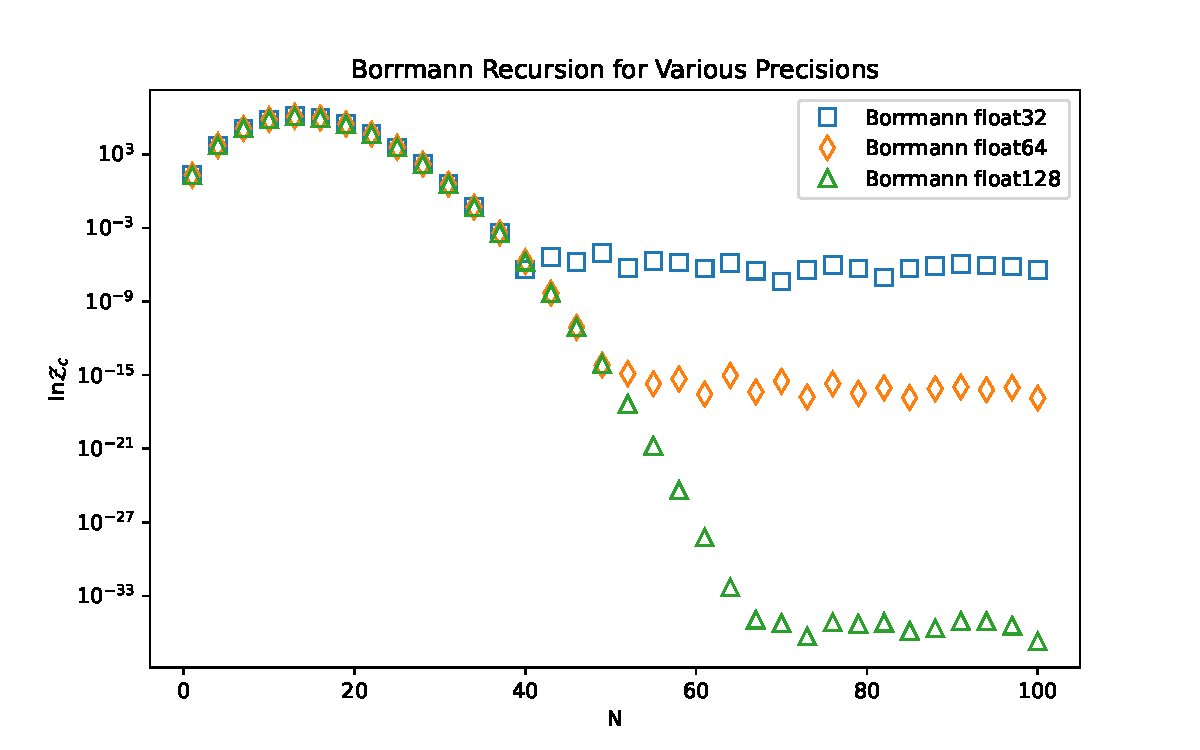
\includegraphics[scale=0.6]{figures/pdf/Borrmann accuracy.pdf}
    \caption{The solution for the Borrman recursive relation of the canonical partition function for different machine precisions. As $N$ increases, the required precision to accurately find the partition function also increases. The breakdown of the recursion is only delayed by the precision used. Therefore, this is numerically expensive to calculate for $N>60$. Figure adapted from \cite{Jiang}.}
    \label{fig:BorrmannAcc}
\end{figure}
As shown, to accurately calculate the partition function, the summation must either be truncated before it fails or the numerical precision used must be increased. The latter method becomes very computationally expensive from a memory standpoint and takes a long time. 
In addition to this, the $(-1)^{k+1}$ term creates another problem. This term means that the summation is constantly changing signs creating a sort of sign problem. Once again, fixing this problem requires truncation or an increase in numerical precision. Truncating the summation may fail to completely describe the partition function and higher precision requires more memory. Given these problems, it is necessary to use a different approach. 

Instead of using this general recursive relation, it is helpful to see if there are any specific cases that can be solved. The easiest example would be that of fermions confined in a harmonic trap. An exact solution was found for this spectrum by Sch\"onhammer \cite{Schon1996}. For the one dimensional simple harmonic oscillator, the partition function was found to be
\begin{equation}
    Z_N=e^{-\beta E_N^0} \prod_{m=1}^N \frac{1}{1-e^{-\beta m\Delta}} \label{schoneqn}
\end{equation}
where $\Delta$ is the spacing between equidistant energy levels and $E_N^0$ is the ground state energy \cite{Schon1996}. This is the exact solution for the canonical partition function of a linear spectrum and provides a result that other methods can use to check their accuracy.

While this solution works for the specific cases of a linear energy spectrum, a general solution is still needed for other energy spectra. This has been worked out by Barghathi et al. \cite{Hatem2020}. The canonical partition function can be calculated using a summation.
\begin{equation}
    Z_N=\sum_{k=k_{min}}^{k_{max}} Z_k(S^{(1)})Z_{N-k}(S^{(2)})
    \label{eq:ZNcombine}
\end{equation}
where $S$ denotes a spectrum that is a union of disjoint subspectra \cite{Hatem2020}. This can be written as 
\begin{gather}
    S=S^{(1)}\cup S^{(2)}.
\end{gather}
Using this spectral formulation, the partition function summation can be written more specifically as 
\begin{equation}
    Z_N=\sum_{k=0}^N Z_k(\{\epsilon_1,\epsilon_2,...\epsilon_j\})Z_{N-k}^{\backslash \{\epsilon_1,\epsilon_2,...\epsilon_j\}} \label{newZN}
\end{equation}
where the $\backslash \{\epsilon_1,\epsilon_2,...\epsilon_j\} $ denotes the energy levels excluded from the spectrum of the particular partition function. Now let each spectrum $S^{(j)}$ consist of a single energy level. For non-interacting fermions, the partition function of a system with a single energy level is
\begin{equation}
    Z_k(\{j\})=\begin{cases} e^{-\beta \epsilon_j k} & 0\leq k \leq 1\\0 & \text{otherwise}.\end{cases}
\end{equation}
By substituting this into Eq.\@ (\ref{newZN}) we see that
\begin{equation}
    Z_N=Z_N^{\backslash\{j\}}+e^{-\beta\epsilon_j}Z_{N-1}^{\backslash\{j\}}. \label{hatemrr}
\end{equation}
This equation can be understood by looking at each term on the right side. On the left side of the addition, the $Z_N^{\backslash\{j\}}$ term is the canonical partition function of $N$ particles with no particle in the $j$th energy level. This represents the complementary probability, or the probability that energy level $\epsilon_j$ is unoccupied. The term on the right hand side has a Boltzmann probability for energy level $\epsilon_j$ times the canonical partition function of $N-1$ particles with no particle at the $j$th energy level. The Boltzmann term introduces the probability of occupying state $j$ with a particle, so the total number of particles on the right hand side of the addition is $N$, the same as the left. The state that is excluded from the partition function is reintroduced meaning that this term is the probability that energy level $\epsilon_j$ is occupied. Since the state can only be occupied or unoccupied for fermions, we can recognize that the full partition function is a sum of the unoccupied and occupied terms, or the full probability. 

To understand this better, let's consider another simple example with only two energy levels $\epsilon_1$ and $\epsilon_2$. The canonical partition functions is 
\begin{equation}
    Z_N = \begin{cases}
    1 & N=0\\
    e^{\epsilon_1}+e^{\epsilon_2} & N=1\\
    e^{\epsilon_1+\epsilon_2} & N=2
    \end{cases}.
\end{equation}
Now using this formulation from above, break down the full spectrum into two subsectra given as 
\begin{gather}
    Z_N^1=\begin{cases}1&N=0\\e^{\epsilon_1}& N=1\end{cases}\\
    Z_N^2=\begin{cases}1&N=0\\e^{\epsilon_2}& N=1\end{cases}.
\end{gather}
Now the partition function corresponding to each $N$ can be calculated using Equation (1.35)  
\begin{gather}
    Z_0= (1)(1)=1\\
    Z_1= (1)(e^{-\beta\epsilon_1})+(e^{-\beta\epsilon_2})(1)=e^{-\beta\epsilon_1}+e^{-\beta\epsilon_2}\\
    Z_2=(e^{-\beta\epsilon_1})(e^{-\beta\epsilon_2})=e^{-\beta\epsilon_1-\beta\epsilon_2}.
\end{gather}
Putting these values together yields 
\begin{equation}
    Z_N = \begin{cases}
    1 & N=0\\
    e^{\epsilon_1}+e^{\epsilon_2} & N=1\\
    e^{\epsilon_1+\epsilon_2} & N=2
    \end{cases}.
\end{equation}
which is exactly what was calculated before. So the canonical partition function can indeed be found through this method.
    \chapter{Relevant Theory} \label{ch:ns-equations}
\begin{em}
The methods shown in the previous section describe recursive relationships that build the canonical ensemble. Some of these are numerically unstable while others only apply to a specific spectrum. In an effort to fix these issues, a method that utilizes the grand canonical ensemble will be developed. First, this requires some connection between the canonical and grand canonical ensembles. This connection will be developed in the following section and used to find the occupation probability and extract the temperature. Finally, degenerate spectra will be considered and their error in temperature measurements will be calculated.  
\end{em}
\section{Connecting the Ensembles}
To find a connection between the grand canonical and canonical ensembles, let us return to the partition functions and occupation probabilities discussed in Section 1.2. To begin, consider Equation (1.6) which connects the two ensembles together as 
\begin{equation*}
    Z_{GC}=\sum_{N=0}^{\infty} e^{\beta\mu N} Z_{N}.
\end{equation*}
Using the same idea as Equation (1.9), the probability of being in a single arbitrary state $N$ is 
\begin{equation}
    \avg{p_N}=\frac{e^{\beta\mu N} Z_N}{Z_{GC}}=P(N).
\end{equation}
This equation can be adjusted to read as
\begin{equation}
    Z_N=P(N) Z_{GC} e^{-\beta\mu N}.
\end{equation}
So now there is a connection between the two ensembles. The last two terms make sense in that the difference between the two ensembles is the addition of the chemical potential term. The only term missing is $P(N)$. This is the probability that the grand canonical partition function describes the canonical partition function with $N$ particles. To find this term requires looking more at Equation (2.1).

\section{Poisson Binomial Recursion Relation}
In order to find the probability distribution, $P(N)$, Equation (1.37) needs to be developed further. Rewritten Equation (2.1) using the relationship in Equation (1.12) produces
\begin{equation}
    P(N)=\frac{Z_n e^{\beta\mu N}}{Z_{GC}}=\frac{Z_N e^{\beta\mu N}}{\prod_k \frac{1}{q_k}}= Z_N e^{\beta\mu N} \prod_k q_k.
\end{equation}
From this, a change of variable will be made such that 
\begin{gather}
    \Tilde{Z}_N = B^N Z_N \prod_k A_k\\
    Z_N=\frac{\Tilde{Z}_N}{B^N \prod_k A_k}.
\end{gather}
The values for $B^N$ and $\prod_k A_k$ are $B^N=e^{\beta\mu N}$ and $\prod_k q_k$ from Equation (2.3). They will be used later, but for now Equation (2.5) can be plugged directly into Equation (1.37) to get
\begin{equation}
    Z_N=\frac{\Tilde{Z}_N}{B^N \prod_k A_k} = \frac{\Tilde{Z}_N^{\backslash\{j\}}}{\frac{B^N}{A_j} \prod_k A_k}+e^{-\beta\epsilon_j}\frac{\Tilde{Z}_{N-1}^{\backslash\{j\}}}{\frac{B^{N-1}}{A_j} \prod_k A_k}.
\end{equation}
An important note here is that the division by $A_j$ is to account for the missing energy level $j$. Also, the exponent on the $B$ terms correspond to the number of particles being considered in the original $Z_N^{\backslash\{j\}}$ term. Simplifying this expression gives
\begin{equation}
   \Tilde{Z}_N=A_j \Tilde{Z}_N^{\backslash\{j\}}+ e^{-\beta\epsilon_j} B \Tilde{Z}_{N-1}^{\backslash\{j\}} A_j.
\end{equation}
Now the corresponding values of $A$ and $B$ can be used to produce
\begin{align}
    \Tilde{Z}_N&=q_j \Tilde{Z}_N^{\backslash\{j\}}+ e^{-\beta\epsilon_j} q_j e^{\beta\mu} \Tilde{Z}_{N-1}^{\backslash\{j\}}\nonumber\\
    &=q_j \Tilde{Z}_N^{\backslash\{j\}}+ e^{-\beta(\epsilon_j-\mu)} (1-p_j) \Tilde{Z}_{N-1}^{\backslash\{j\}}\nonumber\\
    &=q_j \Tilde{Z}_N^{\backslash\{j\}}+ e^{-\beta(\epsilon_j-\mu)} \qty(1-\frac{1}{1+e^{\beta(\epsilon_j-\mu)}}) \Tilde{Z}_{N-1}^{\backslash\{j\}}\nonumber\\
    &=q_j \Tilde{Z}_N^{\backslash\{j\}}+ \frac{e^{-\beta(\epsilon_j-\mu)}}{1+e^{-\beta(\epsilon_j-\mu)}} \Tilde{Z}_{N-1}^{\backslash\{j\}}\nonumber\\
    &=q_j \Tilde{Z}_N^{\backslash\{j\}}+ \frac{1}{1+e^{\beta(\epsilon_j-\mu)}} \Tilde{Z}_{N-1}^{\backslash\{j\}}\nonumber\\
    &=q_j \Tilde{Z}_N^{\backslash\{j\}}+ p_j \Tilde{Z}_{N-1}^{\backslash\{j\}}
\end{align}
where $p_j$ is the grand canonical occupation probability and $q_j$ is its compliment. This is a formula to recursively build up $\Tilde{Z}_N$. Next, the definition of $\Tilde{Z}_N$ is found by plugging in the values for $B$ and $A_k$ back into Equation (2.4) to find
\begin{align}
    \Tilde{Z}_N=Z_N B^N \prod_k A_k=Z_N e^{\beta\mu N} \prod_i q_i=\frac{e^{\beta\mu N}Z_N}{Z_{GC}}=P(N).
\end{align}
Plugging this result into (2.8) gives the recursion relationship as
\begin{gather}
    \Tilde{Z}_N=q_j \Tilde{Z}_N^{\backslash\{j\}}+ p_j \Tilde{Z}_{N-1}^{\backslash\{j\}}\\
    P_N=q_j P_N^{\backslash\{j\}}+ p_j P_{N-1}^{\backslash\{j\}}\\
    P_j(N)=q_j P_j(N)+p_j P_{j-1}(N-1)
\end{gather}
where the final step is performed to simplify notation for later. This is the missing probability distribution needed in Equation (2.2). Moreover, there is now a recursive method to find the probability that the grand canonical partition function accurately represents a canonical partition function of $N$ particles. This recursion has many interesting properties. To start, it adds on a value to the distribution each iteration. When at position $N+1$, the $p_j P_{N-1}^{\backslash\{j\}}$ term still contributes a nonzero value to the probability. This means that iterating over all possible $j$ values for $p$ and $q$ will give a distribution that is $N$ values long. This can be viewed in the form of a triangle where the base is constantly extended with each iteration. This creates a sort of pascal triangle. To build some intuition of this, let us consider another short example. To start, let the probability distribution and it's compliment be
\begin{gather}
    p=\qty[1,\frac{1}{2},\frac{1}{3},\frac{1}{6}]\nonumber\\
    q=1-p=\qty[1,\frac{1}{2},\frac{2}{3},\frac{5}{6}]\nonumber.
\end{gather}
where each term in the array corresponds to the probability that a particle occupies (or doesn't occupy) that state. By summing the values in the probability distribution, the total number of particles is expected to be 2. From here, the recursive relationship can be initialized with a value of $P_0(1)=0$. The calculation can then continue until all values in the probability distribution are used. This is done to show
\begin{gather*}
    P_1(1)=p_1 P_{0}(0)+q_1 P_{0}(1)=(1)(0)+(0)(1)=0\\
    P_1(2)=p_1 P_{0}(1)+q_1 P_{0}(2)=(1)(1)+(0)(0)=1\\
    P_1=[0,1]\\
    P_2(1)=p_2 P_{1}(0)+q_2 P_{1}(1)=\qty(\frac{1}{2})(0)+\qty(\frac{1}{2})(0)=0\\
    P_2(2)=p_2 P_{1}(1)+q_2 P_{1}(2)=\qty(\frac{1}{2})(0)+\qty(\frac{1}{2})(1)=\frac{1}{2}\\
    P_2(3)=p_2 P_{1}(2)+q_2 P_{1}(3)=\qty(\frac{1}{2})(1)+\qty(\frac{1}{2})(0)=\frac{1}{2}\\
    P_2=\qty[0,\frac{1}{2},\frac{1}{2}]\\
    P_3(1)=p_3 P_{2}(0)+q_3 P_{2}(1)=\qty(\frac{2}{3})(0)+\qty(\frac{1}{3})(0)=0\\
    P_3(2)=p_3 P_{2}(1)+q_3 P_{2}(2)=\qty(\frac{2}{3})\qty(\frac{1}{2})+\qty(\frac{1}{3})(0)=\frac{1}{3}\\
    P_3(3)=p_3 P_{2}(2)+q_3 P_{2}(3)=\qty(\frac{2}{3})\qty(\frac{1}{2})+\qty(\frac{1}{3})\qty(\frac{1}{2})=\frac{1}{2}\\
    P_3(4)=p_3 P_{2}(4)+q_3 P_{2}(4)=\qty(\frac{2}{3})(0)+\qty(\frac{1}{3})\qty(\frac{1}{2})=\frac{1}{6}\\
    P_3=\qty[0,\frac{1}{3},\frac{1}{2},\frac{1}{6}]\\
    P_4(1)=p_4 P_{3}(0)+q_4 P_{3}(1)=\qty(\frac{5}{6})(0)+\qty(\frac{1}{6})(0)=0\\
    P_4(2)=p_4 P_{3}(1)+q_4 P_{3}(2)=\qty(\frac{5}{6})\qty(\frac{1}{3})+\qty(\frac{1}{6})(0)=\frac{10}{36}\\
    P_4(3)=p_4 P_{3}(2)+q_4 P_{3}(3)=\qty(\frac{5}{6})\qty(\frac{1}{2})+\qty(\frac{1}{6})\qty(\frac{1}{3})=\frac{17}{36}\\
    P_4(4)=p_4 P_{3}(4)+q_4 P_{3}(4)=\qty(\frac{5}{6})\qty(\frac{1}{6})+\qty(\frac{1}{6})\qty(\frac{1}{2})=\frac{8}{36}\\
    P_4(5)=p_4 P_{3}(4)+q_4 P_{3}(4)=\qty(\frac{5}{6})(0)+\qty(\frac{1}{6})\qty(\frac{1}{6})=\frac{1}{36}\\
    P_4=\qty[0,\frac{10}{36},\frac{17}{36},\frac{8}{36},\frac{1}{36}].
\end{gather*}
This solution can be visualized as a triangle as seen in Fig.(2.1). 
\begin{figure}[H]
    \centering
    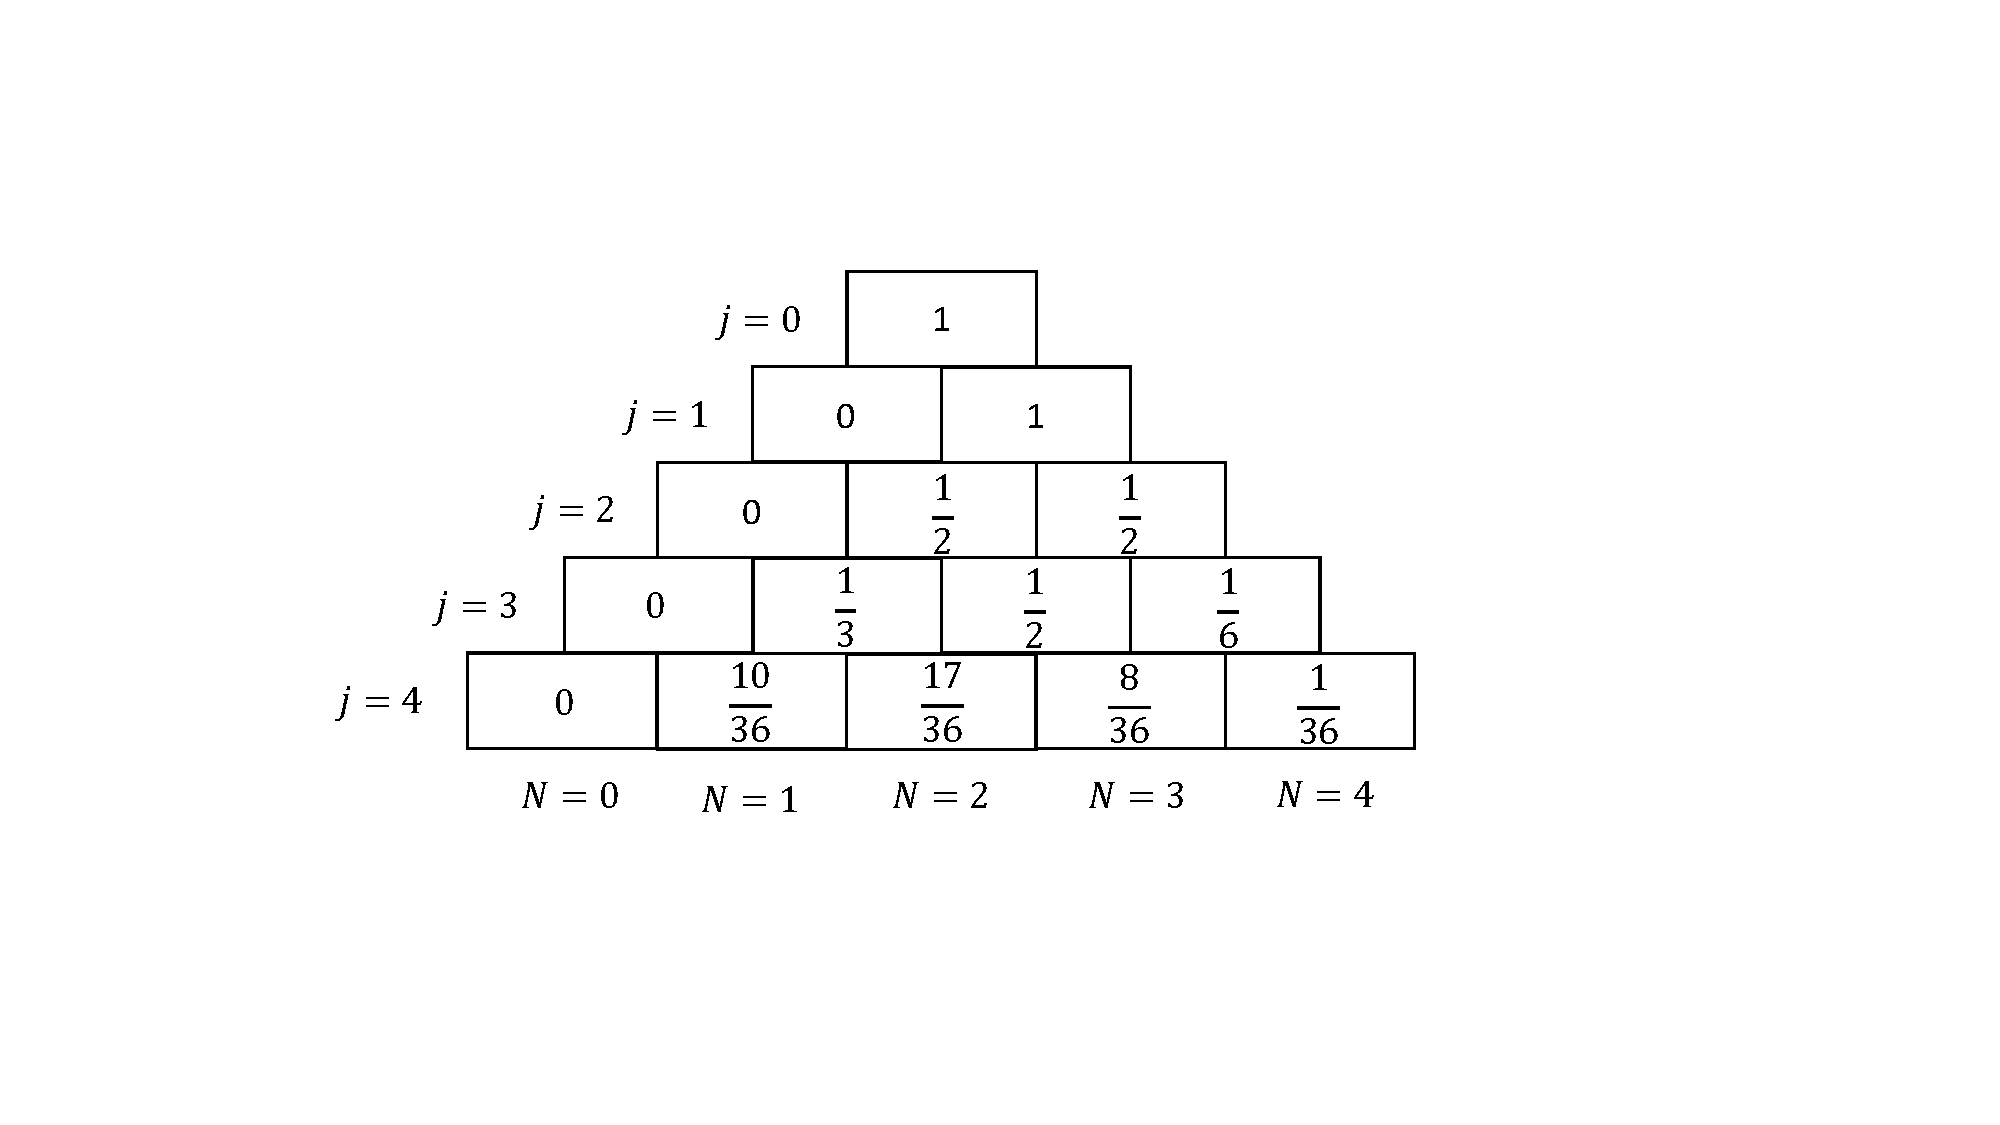
\includegraphics[scale=0.55]{figures/pdf/PBTriangle.pdf}
    \caption{Poisson Binomial Triangle.}
    \label{fig:Poisson Binomial Triangle}
\end{figure}
A more general visualization of this triangle can be seen in Fig.(2.2)
\begin{figure}[H]
    \centering
    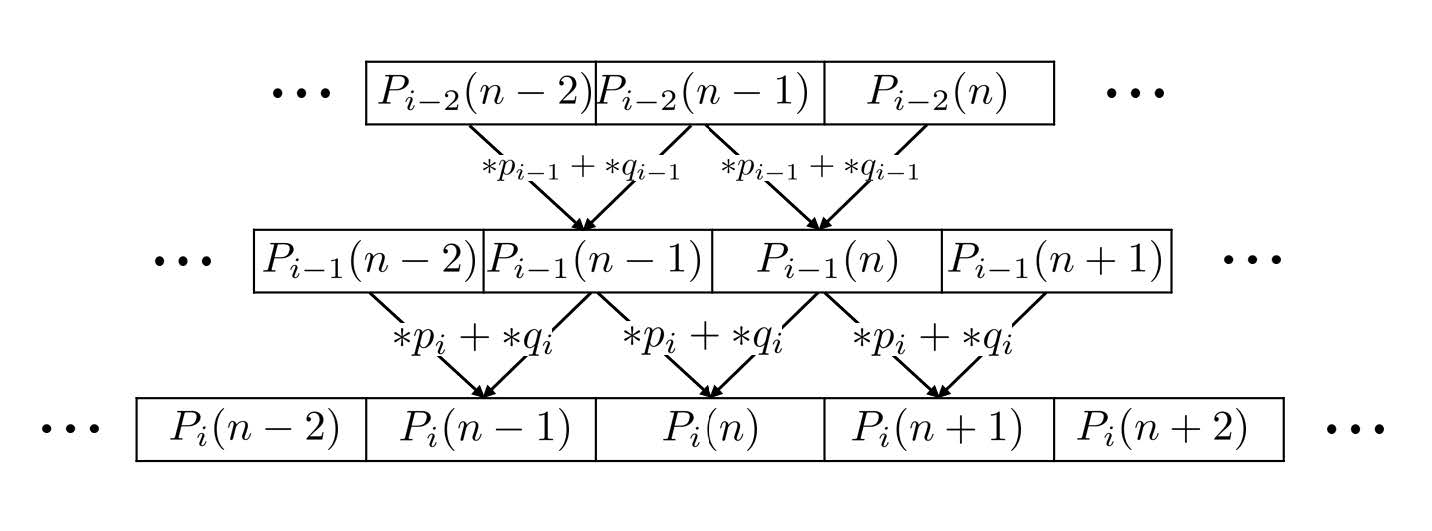
\includegraphics[scale=0.8]{figures/pdf/PBrecursion.jpg}
    \caption{General Poisson Binomial Recursion}
    \label{fig:General Poisson Binomial Recursion}
\end{figure}
As expected, the highest probability corresponds to having $N=2$ particles. Another nice feature of this method is that the probability is normalized. Equation (1.37) has no normalization condition or any reason to be normalized given that the canonical partition function's only restriction is on the number of particles.


\section{Occupation Probability from recursion}
The occupation probability for the canonical ensemble can now be calculated from the Equation (2.12). Rewriting this equation gives
\begin{equation}
    1=\frac{q_j P_{j-1}(N)}{P_j(N)} + \frac{p_j P_{j-1}(N-1)}{P_j(N)}.
\end{equation}
Inspecting this equation, the right fraction is the probability of occupying energy level $j$ and $N-1$ other energy levels. The left fraction is the probability of not occupying energy level $j$ and $N$ other energy levels. This explanation follows from the same idea as the two parts of Equation (1.37). Therefore, the occupation probability for the canonical ensemble is the right fraction on the right hand side of Equation (2.13). Specifically,
\begin{equation}
    \avg{n}_j=\frac{p_j P_{j-1}(N-1)}{P_j(N)}.
\end{equation}

\section{Temperature Extraction}
The occupation probability can now be used to find the correct temperature of the system. To do this, the value of $\beta$ in the original probability distribution is varied until it matches the calculated canonical occupation probability. To do this, the function 
\begin{equation}
    \chi^2=\sum_j(p_j-n_j)^2
\end{equation}
is implemented. The choice of the occupation probability $p$ is of the form of Equation (1.16). The $\mu$ term is set so that the sum of all probabilities equals the number of particles in the system. Therefore, the only term that can be tuned is the temperature dependence of $p_j$, which is $\beta^*$. Since it is dependent only on $\beta^*$, the first and second derivatives can be calculated and used to find the minimum. This is fully calculated in Appendix B, but the important results are 
\begin{gather}
    \frac{d\chi^2}{d\beta^*}=\sum_j -2(p_j-n_j)p_j q_j \epsilon_j+\sum_j 2(p_j-n_j)p_j q_j C_1\\
    \frac{d^2\chi^2}{d\beta^{*2}}=2\sum_j\Biggr[(\epsilon_j-C_1)^2[(p_j-n_j)p_jq_j(q_j-p_j)+p_j^2q_j^2]\nonumber\\
    \ \ \ \ \ \ +(p_j-n_j)p_jq_j(C_1C_3+C_2)\Biggr]\\
    C_1=\frac{\sum_j \epsilon_j p_j q_j}{\sum_j p_j q_j}\\
    C_2=\frac{\sum_j \epsilon_j p_j q_j(p_j - q_j)(\epsilon_j-C_1)}{\sum_j p_j q_j}\\
    C_3=\frac{\partial C_1}{\partial y}=\frac{\partial}{\partial 
    y}\qty{\frac{\sum_j \epsilon_j q_j p_j}{\sum_j p_j q_j}}=\frac{\sum_j p_j q_j(q_j-p_j)(\epsilon_j-C_1)}{\sum_j p_j q_j}.
\end{gather}
With both derivatives available, Newton's method of optimization can be used to find the correct value of $\beta^*$. This method involves using 
\begin{equation}
    \beta^*=\beta^*-\frac{\partial_{\beta^*}\chi^2}{\partial^2_{\beta^*}\chi^2}
\end{equation}
to iterate through the $\chi^2$ function until the minimum is found.

\section{Degenerate energy spectra}
Now the case of degenerate energy spectra will be considered. To begin, define the degeneracy of a certain energy level $i$ as $g_i$. The canonical partition function is written as
\begin{equation}
    Z_k(\epsilon_i;g_i)={g_i \choose k} e^{-k\beta\epsilon_i}
\end{equation}
with $k$ being the number of particles at level $i$.  For the purpose of this calculation, $\beta$ is sufficiently large so that the only excitations will be around Fermi energy level. In this scenario, there are two cases of interest. These are when the degenerate Fermi level is filled and partially filled. 
\subsection{Filled Degenerate Fermi Level}
The first case to consider is when the Fermi level is degenerate and filled. In this case, there are only two levels to worry about, the Fermi level and the first excited state. All other levels are filled or empty. To begin, let $i=0$ denote the Fermi level and $i=1$ denote the first excited state. Since these two levels are the only ones of interest, the simple example in Section 1.3 can be revisited. Consider there is one particle in a system where the Fermi level has degeneracy $g_0$ and energy $\epsilon_0$ and the first excited state has degeneracy $g_1$ and energy $\epsilon_1$. For convenience, the energy spectrum can be redefined as
\begin{equation}
    \epsilon_0 \xrightarrow[]{} 0\ \ \ \ \ \epsilon_1\xrightarrow[]{}\Delta_0=\epsilon_1-\epsilon_1.\nonumber
\end{equation}
The partition function for this case can be written from (1.32) to yield
\begin{align}
    Z_{g_0}(0,\Delta_0;g_0,g_1)&=\sum_{k=0}^{\text{min}(g_1,g_0)} Z_k(\Delta_0,g_1)Z_{g_0-k}(0,g_0)\nonumber\\
    &=\sum_{k=0}^{\text{min}(g_1,g_0)} {g_1 \choose k}{g_0\choose g_0-k} e^{-\beta \epsilon_0 k}e^{-\beta \epsilon_1 k}\nonumber\\
    &=\sum_{k=0}^{\text{min}(g_1,g_0)} {g_1 \choose k}{g_0\choose g_0-k} e^{-\beta \Delta_0 k}
\end{align}
where the $\text{min}(g_1,g_0)$ represents the minimum of the two values. The minimum is used here because there can only be as many particles as there are available positions in the energy level. For non degenerate case, this would be one, but for the degenerate case, this can be an arbitrary positive integer value. The canonical occupation probability can be calculated the same as before by leaving out an energy level and multiplying by its Boltzmann factor. This results in 
\begin{align}
    \avg{n_0}_{g_0}&=\frac{e^{-\beta \epsilon_0}Z_{g_0-1}(0,\Delta_0;g_0-1,g_1)}{Z_{g_0}(0,\Delta_0;g_0,g_1)}\nonumber\\
    &=\frac{\sum_{k=0}^{\text{min}(g_1,g_0-1)} {g_1 \choose k}{g_0\choose g_0-1-k} e^{-\beta \Delta_0 k}}{\sum_{k=0}^{\text{min}(g_1,g_0)} {g_1 \choose k}{g_0\choose g_0-k} e^{-\beta \Delta_0 k }}\nonumber\\
    &=\frac{{g_1\choose 0}{g_0-1\choose g_0-1}+{g_1 \choose 1}{g_0-1\choose g_0-2}e^{-\beta\Delta_0}+{g_1\choose 2}{g_0-1\choose g_0-3}e^{-2\beta\Delta_0}+...}{{g_1\choose 0}{g_0\choose g_0}+{g_1 \choose 1}{g_0\choose g_0-1}e^{-\beta\Delta_0}+{g_1\choose 2}{g_0-1\choose g_0-2}e^{-2\beta\Delta_0}+...}\nonumber\\
    &=\frac{1+g_1(g_0-1)e^{-\beta\Delta_0}+\frac{g_1(g_1-1)(g_0-1)(g_0-2)}{4}e^{-2\beta\Delta_0}+...}{1+g_0g_1e^{-\beta\Delta_0}+\frac{g_1(g_1-1)g_0(g_0-1)}{4}e^{-2\beta\Delta_0}+...}.
\end{align}
Similarly, for the first excited state,
\begin{align}
    \avg{n_1}_{g_0}&=\frac{e^{-k\epsilon_1} Z_{g_0-1}(0,\Delta_0;g_0,g_1-1)}{Z_{g_0}(0,\Delta_0;g_0,g_1)}\nonumber\\
    &=\frac{e^{-k\Delta_0}\sum_{k=0}^{\text{min}(g_1-1,g_0-1)} {g_1-1\choose k}{g_0 \choose k+1} e^{-k\beta\Delta_0}}{\sum_{k=0}^{\text{min}(g_1,g_0)} {g_1\choose k}{g_0 \choose k} e^{-k\beta\Delta_0}}\nonumber\\
    &=\frac{{g_1-1\choose 0}{g_0\choose 1} e^{-\beta\Delta_0} +{g_1-1\choose 1}{g_0\choose 2} e^{-2\beta\Delta_0}+{g_1-1\choose 2}{g_0\choose 3}e^{-3\beta\Delta_0}+...}{{g_0\choose 0}{g_1\choose 0}+{g_0\choose 1}{g_1\choose 1}e^{-\beta\Delta_0}+{g_0\choose 2}{g_1\choose 2}e^{-2\beta\Delta_0}+...}\nonumber\\
    &=\frac{g_0e^{-\beta\Delta_0}+\frac{(g_1-1)g_0(g_0-1)}{2}e^{-2\beta\Delta_0}+...}{1+g_0g_1 e^{-\beta\Delta_0}+\frac{g_1(g_1-1)g_0(g_0-1)}{4}e^{-2\beta\Delta_0}+...}.
\end{align} 
Like before, the chemical potential can be found by using the grand canonical probabilities $p_0$ and $p_1$ such that,
\begin{gather}
    p_0=\frac{1}{1+e^{\beta^*(\epsilon_0-\mu)}}=\frac{1}{1+e^{-\beta^* \mu}}\\
    p_1=\frac{1}{1+e^{\beta^*(\epsilon_0-\mu)}}=\frac{1}{1+e^{\beta^*(\Delta_0-\mu)}}\\
    p_0g_0+p_1g_1=g_0.
\end{gather}
Plugging everything in gives
\begin{gather}
    g_0=\frac{g_0}{1+e^{\beta^*(\epsilon_0-\mu)}}=\frac{1}{1+e^{-\beta^*\mu}}+\frac{g_1}{1+e^{\beta^*(\epsilon_0-\mu)}}=\frac{1}{1+e^{\beta^*(\Delta_0-\mu)}}\nonumber\\
    1+e^{\beta^*\Delta_0} e^{-\beta^*\mu}+\frac{g_1}{g_0}(1+e^{-\beta^*\mu})=(1+e^{-\beta^*\mu})(1+e^{\beta^*\Delta_0} e^{-\beta^* \mu})\nonumber\\
    1+e^{-\beta^*\mu}(\frac{g_1}{g_0}+e^{\beta^*\Delta_0})+\frac{g_1}{g_0}=1+e^{-\beta^*\mu}+e^{\beta^*\Delta_0}e^{-\beta^*\mu}+e^{-2\beta^*\mu}e^{\beta^*\Delta_0}\nonumber\\
    0=(e^{-\beta^*\mu})^2 e^{\beta^*\Delta_0} +e ^{-\beta^*\mu}(1-\frac{g_1}{g_0})-\frac{g_1}{g_0}.
\end{gather}
This is a simple quadratic equation so there will be two solutions. To have a real solution, the positive root is kept resulting in
\begin{align}
    e^{-\beta^*\mu}&=\frac{(\frac{g_1}{g_0}-1)\pm\sqrt{(\frac{g_1}{g_0}-1)^2+4e^{\beta^*\Delta_0}\frac{g_1}{g_0}}}{2e^{\beta^*\Delta_0}}\nonumber\\
    &=\frac{e^{-\beta^*\Delta_0}}{2}(\frac{g_1}{g_0}-1)\pm \frac{1}{2}\sqrt{e^{-2\beta^*\Delta_0} (\frac{g_1}{g_0}-1)^2+ 4e^{-\beta^*\Delta_0}\frac{g_1}{g_0}}.
\end{align}
Just like the simple example before, set the canonical and grand canonical probabilities to be equal, such that $\avg{n_0}_{g_0}=p_0$. This gives 
\begin{align}
    \frac{1}{\avg{n_0}_{g_0}}-1=\frac{1}{p_0}-1=1+e^{-\beta^*\mu}-1=e^{-\beta^*\mu} .
\end{align}
Now there is a connection to the grand canonical probability to the canonical probability for the degenerate case. Setting the two $e^{-\beta^*\mu}$ terms equal to one another yields
\begin{gather}
    \frac{1}{\avg{n_0}_{g_0}}-1=\frac{e^{-\beta^*\Delta_0}}{2}(\frac{g_1}{g_0}-1)\pm \frac{1}{2}\sqrt{e^{-2\beta^*\Delta_0} (\frac{g_1}{g_0}-1)^2+ 4e^{-\beta^*\Delta_0}\frac{g_1}{g_0}}\nonumber\\
    2\frac{1-\avg{n_0}_{g_0}}{\avg{n_0}_{g_0}}-e^{-\beta^*\Delta_0}(\frac{g_1}{g_0}-1)=\sqrt{e^{-2\beta^*\Delta_0} (\frac{g_1}{g_0}-1)^2+ 4e^{-\beta^*\Delta_0}\frac{g_1}{g_0}}\nonumber\\
    4\qty(\frac{1-\avg{n_0}_{g_0}}{\avg{n_0}_{g_0}})^2-4e^{-\beta^*\Delta_0}\qty(\frac{g_1}{g_0}-1) \frac{1-\avg{n_0}_{g_0}}{\avg{n_0}_{g_0}}+e^{-2\beta^*\Delta_0} \qty(\frac{g_1}{g_0}-1)^2\nonumber\\ 
    \ \ \ \ \ \ \  =e^{-2\beta^*\Delta_0} (\frac{g_1}{g_0}-1)^2+ 4e^{-\beta^*\Delta_0}\frac{g_1}{g_0} \nonumber\nonumber\\
    0=4\qty(\frac{1-\avg{n_0}_{g_0}}{\avg{n_0}_{g_0}})^2- 4e^{-\beta^*\Delta_0}\qty(\qty(\frac{g_1}{g_0}-1)\frac{1-\avg{n_0}_{g_0}}{\avg{n_0}_{g_0}}+\frac{g_1}{g_0})\nonumber\\
    4\qty(\frac{1-\avg{n_0}_{g_0}}{\avg{n_0}_{g_0}})^2=4e^{-\beta^*\Delta_0}\qty(\qty(\frac{g_1}{g_0}-1)\frac{1-\avg{n_0}_{g_0}}{\avg{n_0}_{g_0}}+\frac{g_1}{g_0})\nonumber\\
    e^{\beta^* \Delta_0}=\frac{1-\avg{n_0}_{g_0}}{\avg{n_0}_{g_0}}(\frac{g_1}{g_0}-1)+\qty(\frac{1-\avg{n_0}_{g_0}}{\avg{n_0}_{g_0}})^2\frac{g_1}{g_0}.
\end{gather}
With this definition, $\frac{1-\avg{n_0}_{g_0}}{\avg{n_0}_{g_0}}$ terms are worked out and plugged in. This is done in Appendix C.1. An important note for these calculations is that terms greater than $\mathcal{O}\qty(e^{-2\beta \Delta_0})$ are neglected because they will be sufficiently small. Using Equations (C.8) and (C.9),
\begin{align}
    e^{\beta^* \Delta_0}&=\frac{e^{\beta\Delta_0}}{g_1}\qty(1+\frac{(g_1+1)(g_0-1)}{2}e^{-\beta\Delta_0})\qty(\frac{g_1}{g_0}-1)\nonumber\\
    &\ \ \ \ \ \ \ \ \ \ +\frac{e^{2\beta\Delta_0}}{g_1^2}\qty(1+(g_1+1)(g_0-1)e^{-\beta\Delta_0})\frac{g_1}{g_0}\nonumber\\
    &=\frac{e^{2\beta\Delta_0}}{g_1g_0}\qty((g_1-g_0)e^{-\beta\Delta_0}+f+(g_1+1)(g_0-1)e^{-\beta\Delta_0})\nonumber\\
    &=\frac{e^{2\beta\Delta_0}}{g_1g_0}\qty((g_1g_0-1)e^{-\beta\Delta_0}+1)\\
    \beta^*\Delta_0&=2\beta\Delta_0-\ln(g_0g_1)+\ln\qty((g_1g_0-1)e^{-\beta\Delta_0}+1).
\end{align}
Since $e^{-\beta\Delta_0}$ is small, the third term on the right hand size can be approximated using $\ln(1+x)\approx x$. This yields
\begin{align}
    \beta^*\Delta_0&=2\beta\Delta_0-\ln\qty(g_0g_1)+(g_1g_0-1)e^{-\beta\Delta_0}\nonumber\\
    \beta^*&=2\beta-\frac{\ln\qty(g_0g_1)}{\Delta_0}+\frac{g_1g_0-1}{\Delta_0}e^{-\beta\Delta_0}.
\end{align} 
This is the relationship between the canonical temperature and the grand canonical temperature. This can be rewritten in terms of the error of the grand canonical $\beta^*$ value. For this, consider 
\begin{align}
    \frac{\beta^*-\beta}{\beta}=\frac{\delta\beta}{\beta}=1-\frac{\ln(g_0g_1)}{\beta\Delta_0}+\frac{(g_1g_0 - 1)}{\beta \Delta_0}e^{-\beta\Delta_0}.
\end{align}
To check if this is accurate, this equation should give the same results when the degeneracies are removed.
\begin{gather}
    g_0=g_1=1\nonumber\\
    \frac{\delta\beta}{\beta}=1-\frac{\ln(1)}{C_1}+\frac{(1)(1)-1}{C_2}=1\nonumber
\end{gather}
This is the condition for the nondegenerate case, so the filled degenerate fermi level theory matches the nondegenerate theory. 
\subsection{Partially Filled Degenerate Fermi Level}
Turning to the case of a partially filled degenerate energy spectrum, consider that the Fermi level is partially filled. This setup requires considering both the level above and below the Fermi level. The energy spectrum can be rewritten as 
\begin{gather}
    \epsilon_0 \xrightarrow[]{} 0\nonumber\\
    \epsilon_1 \xrightarrow[]{} \Delta_0=\epsilon_1-\epsilon_0\nonumber\\
    \epsilon_{-1} \xrightarrow[]{} -\Delta_{-1}=\epsilon_{-1}-\epsilon_0.\nonumber
\end{gather}
The number of particles in the partially filled level will be denoted as $\ell$. The partition function for this case is 
\begin{align}
    &Z_{g_{-1}+\ell}(-\Delta_{-1},0,\Delta;g_{-1},g_0,g_1) = e^{g_{-1}\beta\Delta_{-1}} \Biggr[{g_0\choose \ell}+g_1{g_0\choose \ell-1}e^{-\beta\Delta_0} \nonumber\\
    &\quad +g_{-1}{g_0\choose \ell+1}e^{-\beta\Delta_{-1}} +\frac{g_1(g_1-1)}{2} {g_0\choose \ell-2}e^{-2\beta\Delta_0}\nonumber\\ 
    &\quad +\frac{g_{-1}(g_{-1}-1)}{2} {g_0\choose \ell+2} e^{-2\beta\Delta_{-1}} +g_1g_{-1}{g_0\choose \ell} e^{-\beta(\Delta_0+\Delta_{-1})} \Biggr]\nonumber\\
    &\ \ =e^{g_{-1}\beta\Delta_{-1}} {g_0\choose \ell} \Biggr[1+ \frac{g_1 \ell}{g_0-\ell+1} e^{-\beta\Delta_0} +\frac{g_{-1}(g_0-\ell)}{\ell+1} e^{-\beta\Delta_{-1}} \nonumber\\
    &\quad+\frac{g_1(g_1-1)}{2} \frac{\ell(\ell-1)}{(g_0+\ell+1)(g_0+\ell+2)}e^{-2\beta\Delta_0} \nonumber\\
    &\quad+\frac{g_{-1}(g_{-1}-1)}{2} \frac{(g_0-\ell)(g_0-\ell-1)}{(\ell+1)(\ell+2)} e^{-2\beta\Delta_{-1}}+g_1g_{-1}e^{-\beta(\Delta_0+\Delta_{-1})}\Biggr].
\end{align}
As before, the partition function can be found for states with one particle removed. For level $i=-1$,
\begin{align}
    &Z_{g_{-1}+\ell-1}(-\Delta_{-1},0,\Delta_0;g_{-1}-1,g_0,g_1)=e^{(g_{-1}-1)\beta\Delta_{-1}} {g_0\choose \ell} \Biggr[1+\frac{g_1 \ell}{g_0-\ell+1} e^{-\beta\Delta_0} \nonumber\\
    &\quad +\frac{(g_{-1}-1)(g_0-\ell)}{\ell+1} e^{-\beta\Delta_{-1}}+\frac{g_1(g_1-1)}{2} \frac{\ell(\ell-1)}{(g_0+\ell+1)(g_0+\ell+2)}e^{-2\beta\Delta_0} \nonumber\\
    &\quad+\frac{(g_{-1}-1)(g_{-1}-2)}{2} \frac{(g_0-\ell)(g_0-\ell-1)}{(\ell+1)(\ell+2)} e^{-2\beta\Delta_{-1}}+g_1(g_{-1}-1)e^{-\beta(\Delta_0+\Delta_{-1})}\Biggr].
\end{align}
For level $i=0$,
\begin{align}
    &Z_{g_{-1}+\ell-1}(-\Delta_{-1},0,\Delta_0;g_{-1},g_0-1,g_1)=e^{g_{-1}\beta\Delta_{-1}} {g_0-1\choose \ell-1} \Biggr[1+\frac{g_1 (\ell-1)}{g_0-\ell-1} e^{-\beta\Delta_0}\nonumber\\
    &\quad+\frac{g_{-1}(g_0-\ell)}{\ell} e^{-\beta\Delta_{-1}} +\frac{g_1(g_1-1)}{2} \frac{(\ell-1)(\ell-2)}{(g_0+\ell+1)(g_0+\ell+2)}e^{-2\beta\Delta_0}\nonumber\\ &\quad+\frac{g_{-1}(g_{-1}-1)}{2} \frac{(g_0-\ell)(g_0-\ell-1)}{\ell(\ell+1)} e^{-2\beta\Delta_{-1}} +g_1g_{-1}e^{-\beta(\Delta_0+\Delta_{-1})}\Biggr].
\end{align}
For level $i=1$,
\begin{align}
    &Z_{g_{-1}+\ell}(-\Delta_{-1},0,\Delta;g_{-1},g_0,g_1-1) =e^{g_{-1}\beta\Delta_{-1}} {g_0\choose \ell-1} \Biggr[1+\frac{(g_1-1) (\ell-1)}{g_0-\ell-1} e^{-\beta\Delta_0} \nonumber\\
    &\quad+\frac{g_{-1}(g_0-\ell+1)}{\ell} e^{-\beta\Delta_{-1}} +\frac{(g_1-1)(g_1-2)}{2} \frac{(\ell-2)(\ell-3)}{(g_0+\ell+2)(g_0+\ell+3)}e^{-2\beta\Delta_0}\nonumber\\ &\quad+\frac{g_{-1}(g_{-1}-1)}{2} \frac{(g_0-\ell+1)(g_0-\ell)}{(\ell-1)\ell} e^{-2\beta\Delta_{-1}} +g_1g_{-1}e^{-\beta(\Delta_0+\Delta_{-1})}\Biggr].
\end{align}
As before, the grand canonical occupation probability are written as,
\begin{gather}
    p_1=\frac{1}{1+e^{\beta^*(\Delta_1-\mu)}}\nonumber\\
    p_0=\frac{1}{1+e^{-\beta^*\mu}}\nonumber\\
    p_{-1}=\frac{1}{1+e^{\beta^*(\Delta_{-1}-\mu)}}\nonumber
\end{gather}
The chemical potential is found from the particle number. This is worked out in Appendix C.2, but the solution is shown below. 
\begin{align}
    &0=e^{-3\beta^*\mu}(e^{\beta^*(\Delta_1+\Delta_{-1})})\nonumber\\
    &+e^{-2\beta^*\mu}\Biggr(e^{\beta^*\Delta_1}+e^{\beta^*\Delta_{-1}}+e^{\beta^*(\Delta_{-1}+\Delta_1)}-\frac{g_1}{g_{-1}+\ell}e^{\beta^*\Delta_{-1}}\nonumber-\frac{g_0}{g_{-1}+\ell}e^{\beta^*(\Delta_1+\Delta_{-1})}\nonumber\\
    &\quad\quad\quad\quad\ \ \ -\frac{g_{-1}}{g_{-1}+\ell}e^{\beta^*\Delta_1}\Biggr)\nonumber\\
    &+e^{-\beta^*\mu}\Biggr(1+e^{\beta^*\Delta_1}+e^{\beta^*\Delta_{-1}}-\frac{g_1}{g_{-1}+\ell}(1+e^{\beta^*\Delta_{-1}})-\frac{g_0}{g_{-1}+\ell}(e^{\beta^*\Delta_1}+e^{\beta^*\Delta_{-1}})\nonumber\\
    &\quad\quad\quad\quad\ \ -\frac{g_{-1}}{g_{-1}+\ell}(1+e^{\beta^*\Delta_1})\Biggr)\nonumber\\
    & +(1-\frac{g_1}{g_{-1}+\ell}-\frac{g_0}{g_{-1}+\ell}-\frac{g_{-1}}{g_{-1}+\ell})
\end{align}
This is a cubic equation with roots that contain $e^{-\beta^*\Delta_0}$ and $e^{-\beta^*\Delta_{-1}}$. 
Given this equation, there are more variables than equations describing this case, so an exact solution cannot be found. Therefore, it's desirable to turn this into a two level system. To do so, consider that either $\Delta_0$ or $\Delta_{-1}$ is large enough that any excitations to or from that level are negligible. These two cases are discussed in the following sections. 

\subsubsection{Case 1: $\beta^*(\Delta_{-1}-\Delta_0)\gg 1$}
For this case, the gap between the excited state and the Fermi level is much smaller than the gap between the state below and the Fermi level. For this case, the excitations from the $i=-1$ level can be ignored. This brings the problem back to a two level system that can be exactly solved. The occupation probability is then defined as
\begin{align}
    \avg{n_0}_\ell&=\frac{Z_{\ell-1}(0,\Delta_0;g_0-1,g_1)}{Z_\ell(0,\Delta_0;g_0,g_1)}\nonumber\\
    &=\frac{{g_0-1\choose \ell-1}[1+\frac{g_1(\ell-1)}{g_0-\ell+1}e^{-\beta\Delta_0} +\frac{g_1(g_1-1)(\ell-1)(\ell-2)}{2(g_0-\ell+1)(g_0-\ell+2)}e^{-2\beta\Delta_0}]}{{g_0\choose \ell}[1+\frac{g_1 \ell}{g_0-\ell+1}e^{-\beta\Delta_0} +\frac{g_1(g_1-1)\ell(\ell-1)}{2(g_0-\ell+1)(g_0-\ell+2)}e^{-2\beta\Delta_0}]}\nonumber\\
    &=\frac{\frac{\ell}{g_0} [1+\frac{g_1(\ell-1)}{g_0-\ell+1}e^{-\beta\Delta_0} +\frac{g_1(g_1-1)(\ell-1)(\ell-2)}{2(g_0-\ell+1)(g_0-\ell+2)}e^{-2\beta\Delta_0}]}{1+\frac{g_1 \ell}{g_0-\ell+1}e^{-\beta\Delta_0} +\frac{g_1(g_1-1)\ell(\ell-1)}{2(g_0-\ell+1)(g_0-\ell+2)}e^{-2\beta\Delta_0}}.
\end{align}
The approximation $\frac{1}{1+x}\approx 1-x+x^2$ is used. Keeping only leading order terms,
\begin{align}
    \avg{n_0}_\ell&=\frac{\ell}{g_0}\qty[1+\frac{g_1(\ell-1)}{g_0-\ell+1}e^{-\beta\Delta_0} +\frac{g_1(g_1-1)(\ell-1)(\ell-2)}{2(g_0-\ell+1)(g_0-\ell+2)}e^{-2\beta\Delta_0}]\nonumber\\
    &\times \qty[1-\frac{g_1\ell}{g_0-\ell+1}e^{-\beta\Delta_0}-\frac{g_1(g_1-1)\ell(\ell-1)}{2(g_0-\ell+1)(g_0-\ell+2)}e^{-2\beta\Delta_0}+(\frac{g_1 \ell e^{-\beta\Delta_0}}{g_0-\ell+1}+...)^2] \nonumber\\
    &=\frac{\ell}{g_0}\Biggr[1-\frac{g_1\ell}{g_0-\ell+1}e^{-\beta\Delta_0}-\frac{g_1(g_1-1)\ell(\ell-1)}{2(g-\ell+1)(g_0-\ell+2)}e^{-2\beta\Delta_0}+\frac{g_1(\ell-1)}{g_0-\ell+1}e^{-\beta\Delta_0}\nonumber\\
    &-\frac{g_1^2 \ell(\ell-1)}{(g_0-\ell+1)^2}e^{-2\beta\Delta_0}+\frac{g_1(g_1-1)(\ell-1)(\ell-2)}{2(g_0-\ell+1)(g_0-\ell+2)}e^{-2\beta\Delta_0}+\frac{g_1^2\ell^2}{(g_0-\ell+1)^2}e^{-2\beta\Delta_0}\Biggr]\nonumber\\
    &=\frac{\ell}{g}\qty[1-\frac{g_1}{g_0-\ell+1}e^{-\beta\Delta_0}+\frac{g_1(g_0-\ell+1)(g_1+\ell-1)+g_1\ell^2}{(g_0-\ell+1)^2(g_0-\ell+2)}e^{-2\beta\Delta_0}].
\end{align}          
Using the grand canonical probabilities, the chemical potential term can be found from
\begin{equation}
    g_0 p_0+g_1 p_1=\ell.
\end{equation}
This produces a quadratic equation, with the solution
\begin{align}
    e^{-\beta^*\mu }&=\frac{1}{2}((\frac{g_0}{\ell}-1)+(\frac{g_1}{\ell}-1)e^{-\beta^*\Delta_0})\nonumber\\
    &+\frac{1}{2}\sqrt{((\frac{g_0}{\ell}-1)+(\frac{g_1}{\ell}-1)e^{-\beta^*\Delta_0})^2-4e^{-\beta^*\Delta_0}(1-\frac{g_0}{\ell}-\frac{g_1}{\ell})}.
\end{align}
Equation (2.31) is used again to find $\avg{n_0}_{g_0}$ in terms of $e^{-\beta^*\mu}$.
Setting the first term equal to Equation (2.45) gives an equation that can be solved for $e^{-\beta^*\Delta_0}$. This is worked out in Appendix C.3. The solution is
\begin{align}
    e^{-\beta^*\Delta_0}&=\frac{g_0-\ell}{g_0-\ell+1}e^{-\beta\Delta_0} \Biggr[1+\frac{g_1 \ell}{(g_0-\ell)(g_0-\ell+1)}e^{-\beta\Delta_0}\nonumber\\
    &\ \ \ \ \ \ \ \ \ \ \ \ \ \ \ \ \ \ \ +\frac{(g_0-\ell+1)-g_1\ell+g_1+g_0}{(g_0-\ell+1)(g_0-\ell+2)}e^{-\beta\Delta_0}\Biggr]
\end{align}
For a partially filled Fermi level, $g_0\neq \ell$. Keeping only terms to the first order in $e^{-\beta\Delta_0}$, Equation (2.46) becomes
\begin{align}
    e^{-\beta^*\Delta_0}&=\frac{g_0-\ell}{g_0-\ell+1} e^{-\beta\Delta_0}\nonumber\\
    -\beta^*\Delta_0&=-\beta\Delta_0+\ln(\frac{g_0-\ell}{g_0-\ell+1})\nonumber\\
    \beta^*&=\beta+\frac{1}{\Delta_0}\ln(\frac{g_0-\ell+1}{g_0-\ell})\nonumber\\
    \frac{\delta\beta}{\beta}=\frac{\beta^*-\beta}{\beta}&=\frac{1}{\Delta_0 \beta}\ln(\frac{g_0-\ell+1}{g_0-\ell}).
\end{align}
In the case when $g_0=\ell$, the filled degenerate theory should reappear. This requires that the next order be included in Equation (2.46). Since $g_0-\ell=g_0-g_0$, the only term that survives is the second in the bracket. This gives
\begin{align}
    e^{-\beta^*\Delta_0}&= e^{-\beta\Delta_0} \qty(\frac{g_1 \ell}{(g_0-\ell+1)^2} e^{-\beta\Delta_0})\nonumber\\
    &=e^{-2\beta\Delta_0} \frac{g_1 g_0}{(g_0-g_0+1)^2}\nonumber\\
    &=g_0g_1e^{-2\beta\Delta_0}\nonumber\\
    \beta^*\Delta_0&=2\beta\Delta_0 - \ln(g_1g_0)\nonumber\\
    \frac{\delta\beta}{\beta}&=1-\frac{1}{\beta\Delta_0} \ln(g_0g_1).
\end{align}
Checking Equation (2.36), these are the first two terms in the filled degenerate energy spectrum case, so the two theories match. 
\subsubsection{Case 2: $\beta^*(\Delta_0-\Delta_{-1})\gg 1$}
In this case, the gap between the excited state and the Fermi level is much bigger
than the gap between the state below and the Fermi level. Another way to view this case is from the perspective of excitation of holes. When a particle from the state below the Fermi level is excited to the Fermi level, a hole is excited to that lower energy level. Using this formulation, the problem can be reformulated with $\ell \xrightarrow[]{} \Bar{\ell}=g_0-\ell$. Starting again from the grand canonical perspective, the sum of the probability of the two levels should yield the total number of particles between the two levels. Following the previous pattern,
\begin{gather}
    p_0g_0+p_{-1}g_{-1}=g_{-1}+\ell\nonumber\\
    -p_0g_0-p_{-1}g_{-1}=-g_{-1}-\ell\nonumber\\
    g_0(1-p_0)+g_{-1}(1-p_{-1})=-g_{-1}-\ell+g_{-1}+g_0=g_0-\ell\nonumber\\
    g_0\Bar{p}_0+g_{-1}\Bar{p}_{-1}=g_0-\ell=\Bar{\ell}
\end{gather}
where $\Bar{p}_0$ and $\Bar{p}_{-1}$ are the complimentary probabilities. After these substitutions, this equation appears the same as Equation (2.44). The complimentary probabilities can be calculated using the grand canonical picture 
\begin{align}
    \Bar{p}_0&=1-\frac{1}{1+e^{-\beta^*\mu}}=\frac{1}{1+e^{\beta^*\mu}}=\avg{\Bar{n_0}}\\
    e^{\beta^*\mu}&=\frac{1}{\avg{\Bar{n_0}}}-1
\end{align}
where the grand canonical and canonical probabilities are set to equal each other as done before in Equation (2.31). Inspecting this result, the form is the same as Equation (2.31) but now the chemical potential has become negative or $\mu\xrightarrow[]{}-\mu$. This makes sense when remembering that the holes are being considered rather than the particles. The other probability is 
\begin{align}
    \Bar{p}_{-1}&=1-\frac{1}{1+e^{\beta^*(-\Delta_{-1}-\mu)}}=\frac{1}{1+e^{\beta^*(\Delta_{-1}+\mu)}}=\avg{\Bar{n}_{-1}}\\
    e^{\beta^*(\Delta_{-1}+\mu)}&=\frac{1}{\avg{\Bar{n}_{-1}}}-1\nonumber\\
    e^{\beta^*\Delta_{-1}}&=e^{-\beta^*\mu}(\frac{1}{\avg{\Bar{n}_{-1}}}-1)
\end{align}
The relationship from Equation (2.51) can be used to get rid of the chemical potential term above. This yields
\begin{align}
    e^{\beta^*\Delta_{-1}}&=e^{-\beta^*\mu}(\frac{1}{\avg{\Bar{n}_{-1}}}-1)\nonumber\\
    &=\frac{\frac{1}{\avg{\Bar{n}_{-1}}}-1}{\frac{1}{\avg{\Bar{n}_0}}-1}\nonumber\\
    &=\frac{\avg{\Bar{n}_0}(1-\avg{\Bar{n}_{-1}})}{\avg{\Bar{n}_{-1}}(1-\avg{\Bar{n}_0})}.
\end{align}
To write $\avg{\Bar{n}_{-1}}$ in terms of $\avg{\Bar{n}_0}$, the $p_0$ and $p_{-1}$ terms in Equation (2.50) need to be replaced with their canonical ensemble counter part like in Equations (2.51) and (2.53). Doing so gives the following relationship
\begin{gather}
    g_0\Bar{p}_0+g_{-1}\Bar{p}_{-1}-\Bar{\ell}=g_0\avg{\Bar{n}_0}+g_{-1}\avg{\Bar{n}_{-1}}\\
    \avg{\Bar{n}_{-1}}=\frac{\Bar{\ell}}{g_{-1}}-\frac{g_0}{g_{-1}}\avg{\Bar{n}_0}
\end{gather}
Plugging this into Equation (2.54) yields
\begin{align}
    e^{\beta^*\Delta_{-1}}&=\frac{\avg{\Bar{n}_0}(1-\frac{\Bar{\ell}}{g_{-1}}+\frac{g_0}{g_{-1}}\avg{\Bar{n}_0})}{(1-\avg{\Bar{n}_0})(\frac{\Bar{\ell}}{g_{-1}}-\frac{g_0}{g_{-1}}\avg{\Bar{n}_0})}\\
    e^{-\beta^*\Delta_{-1}}&=\frac{(1-\avg{\Bar{n}_0})(\frac{\Bar{\ell}}{g_0}-\avg{\Bar{n}_0})}{\avg{\Bar{n}_0}(\frac{g_{-1}-\Bar{\ell}}{g_0}+\avg{\Bar{n}_0})}
\end{align}
Upon inspection, this is similar to the equation that is solved in Case 1. Specifically, this is similar to Equation (C.16) with the substitutions $\Delta_0\xrightarrow[]{}\Delta_{-1}$, $\ell\xrightarrow[]{}\Bar{\ell}$, $\avg{n_0}\xrightarrow[]{}\avg{\Bar{n}_0}$, $g_1\xrightarrow[]{}g_{-1}$, and $\mu \xrightarrow[]{}-\mu$. The last term that needs to be checked to see if this formulation is similar to Case 1 is the $\avg{\Bar{n}_0}$ term. Expanding this term, 
\begin{align}
    \avg{\Bar{n}_0}&=1-\avg{n_0}=1-\frac{e^{-\beta\epsilon_0}Z_{g_{-1}+\ell-1}}{Z_{g_{-1}+\ell}}\\
    &=\frac{Z_{g_{-1}+\ell}-e^{-\beta (0)}Z_{g_{-1}+\ell-1}}{Z_{g_{-1}+\ell}}=\frac{Z_{g_{-1}+\ell}-Z_{g_{-1}+\ell-1}}{Z_{g_{-1}+\ell}}
\end{align}
where $\epsilon_0$ is set to zero. Substituting the value for $\ell$ into the denominator term gives
\begin{align}
    &Z_{g_{-1}+\ell+1}(-\Delta_{-1},0;g_{-1},g_0-1)=e^{g_{-1}\beta\Delta_{-1}}{g_0-1 \choose \ell-1}\Biggr[1+\frac{g_{-1}(g_0-\ell)}{\ell}e^{-\beta\Delta_{-1}}\nonumber\\
    &\quad+\frac{g_{-1}(g_{-1}-1)(g_0-\ell)(g_0-\ell-1)}{2\ell(\ell+1)}e^{-2\beta\delta_{-1}}\Biggr]\nonumber\\
    &=e^{g_{-1}\beta\Delta_{-1}}{g_0-1 \choose \Bar{\ell}}\qty[1+\frac{g_{-1}\Bar{\ell}}{g_0-\bar{\ell}}e^{-\beta\Delta_{-1}}+\frac{g_{-1}(g_{-1}-1)\Bar{\ell}(\Bar{\ell}-1)}{2(g_0-\Bar{\ell})(g_0-\Bar{\ell}+1)}e^{-2\beta\delta_{-1}}].
\end{align}
Inspecting this equation, the terms in the brackets are similar to Equation (2.40) with $g_1\xrightarrow[]{}g_{-1}$, $\Delta_1\xrightarrow[]{}\Delta_{-1}$, and $\ell \xrightarrow[]{}\bar{\ell}$. Continuing, the second term in the numerator is
\begin{align}
    &Z_{g_{-1}+\ell+1}(-\Delta_{-1},0;g_{-1},g_0-1)=e^{g_{-1}\beta\Delta_{-1}}{g_0-1\choose \ell-1}\Biggr[1+\frac{g_{-1}(g_0-\ell)}{\ell}e^{-\beta\Delta_{-1}}\nonumber\\
    &\quad+\frac{g_{-1}(g_{-1}-1)(g_0-\ell)(g_0-\ell-1)}{2\ell(\ell+1)}e^{-2\beta\Delta_{-1}}\Biggr]\nonumber\\
    &=e^{g_{-1}\beta\Delta_{-1}}{g_0-1\choose \Bar{\ell}} \qty[1+\frac{g_{-1}\Bar{\ell})}{g_0-\Bar{\ell}}e^{-\beta\Delta_{-1}}+\frac{g_{-1}(g_{-1}-1)\Bar{\ell}(\Bar{\ell}-1)}{2(g_0-\Bar{\ell})(g_0-\Bar{\ell}+1)}e^{-2\beta\Delta_{-1}}].
\end{align}
This last line can be rewritten as 
\begin{align}
    &Z_{g_{-1}+\ell+1}(-\Delta_{-1},0;g_{-1},g_0-1)=e^{g_{-1}\beta\Delta_{-1}}{g_0\choose \Bar{\ell}} \frac{g_0-\bar{\ell}}{g_0} \Biggr[1+\frac{g_{-1}\Bar{\ell})}{g_0-\Bar{\ell}}e^{-\beta\Delta_{-1}}\nonumber\\
    &\quad+\frac{g_{-1}(g_{-1}-1)\Bar{\ell}(\Bar{\ell}-1)}{2(g_0-\Bar{\ell})(g_0-\Bar{\ell}+1)}e^{-2\beta\Delta_{-1}}\Biggr].
\end{align}
This is useful for the calculation of the numerator in Equation (2.58). Calculating this term by term in orders of $e^{\beta\Delta_{-1}}$, the first term is the $e^0$ quantities, which is 
\begin{equation}
    1-\frac{g_0-\bar{\ell}}{g_0}=\frac{g_0-g_0+\bar{l}}{g_0}=\frac{\bar{l}}{g_0}.
\end{equation}
The $e^{\beta\Delta_{-1}}$ quantities give
\begin{align}
    \frac{g_{-1}\ell}{g_0-\Bar{\ell}+1}-\frac{g_0-\Bar{\ell}}{g_0}\frac{g_{-1}\bar{\ell}}{g_0-\bar{\ell}}&=\frac{g_{-1}\bar{\ell}}{g_0-\bar{\ell}+1}-\frac{g_{-1}\bar{\ell}}{g_0}\nonumber\\
    &=\frac{g_{-1}g_0\bar{\ell}-g_{-1}\bar{\ell}(g_0-\bar{\ell}+1)}{(g_0-\bar{\ell}+1)g_0}\nonumber\\
    &=\frac{g_{-1}\bar{\ell}(\bar{\ell}-1)}{g_0(g_0-\bar{\ell}+1)}\nonumber\\
    &=\frac{\bar{\ell}}{g_0} \frac{g_{-1}(\bar{\ell}-1)}{g_0-\bar{\ell}+1}.
\end{align}
The $e^{2\beta\Delta_{-1}}$ quantities give
\begin{gather}
    \frac{g_{-1}(g_{-1}-1)\bar{\ell}(\bar{\ell}-1)}{2(g_0-\bar{\ell}+1)(g_0-\bar{\ell}+2}-\frac{g_{-1}(g_{-1}-1)\bar{\ell}(\bar{\ell}-1)}{2g_0(g_0-\bar{\ell}+1)}\nonumber\\
    =\frac{g_{-1}(g_{-1}-1)\bar{\ell}(\bar{\ell}-1)}{2(g_0-\bar{\ell}+1)}[\frac{1}{g_0-\bar{\ell}+2}-\frac{1}{g_0}]\nonumber\\
    =\frac{g_{-1}(g_{-1}-1)\bar{\ell}(\bar{\ell}-1)}{2(g_0-\bar{\ell}+1)}[\frac{g_0-g_0+\bar{\ell}-2}{g_0(g_0-\bar{\ell}+2)}]\nonumber\\
    =\frac{g_{-1}(g_{-1}-1)\bar{\ell}(\bar{\ell}-1)}{2(g_0-\bar{\ell}+1)}[\frac{\bar{\ell}-2}{g_0(g_0-\bar{\ell}+2)}]\nonumber\\
    =\frac{\bar{\ell}}{g_0}\frac{g_{-1}(g_{-1}-1)(\bar{\ell}-1)(\bar{\ell}-2)}{2(g_0-\bar{\ell}+1)(g_0-\bar{\ell}+2)}.
\end{gather}
Bringing all the terms together and cancelling out terms, the value of $\avg{\bar{n}_0}$ is 
\begin{equation}
    \avg{\bar{n}_0}=\frac{\bar{\ell}}{g_0}\frac{1+\frac{g_{-1}(\bar{\ell}-1)}{g_0-\bar{\ell}+1}e^{-\beta\Delta_{-1}}+\frac{g_{-1}(g_{-1}-1)(\bar{\ell}-1)(\bar{\ell}-2)}{2(g_0-\bar{\ell}+1)(g_0-\bar{\ell}+2)}e^{-2\beta\Delta_{-1}}}{1+\frac{g_{-1}\bar{\ell}}{g_0-\bar{\ell}+1}e^{-\beta\Delta_{-1}}+\frac{g_{-1}(g_{-1}-1)\bar{\ell}(\bar{\ell}-1)}{2(g_0-\bar{\ell}+1)(g_0-\bar{\ell}+2)}e^{-2\beta\Delta_{-1}}}
\end{equation}
Inspecting this equation, it matches Equation (2.43) with $\ell\xrightarrow[]{}\bar{\ell}$, $\Delta_0\xrightarrow[]{}\Delta_{-1}$, $g_1\xrightarrow[]{}g_{-1}$, and $\avg{n_0}\xrightarrow[]{}\avg{\bar{n}_0}$. After making the change to these new terms, the calculations following this will be the same as Case 1 following Equation (2.43). Therefore, the equation for $\frac{\delta\beta}{\beta}$ can be read directly from Case 1 with the proper substitutions. This results in the equation 
\begin{equation}
    \frac{\delta\beta}{\beta}=\frac{1}{\beta\Delta_{-1}}\ln(\frac{g_0-\bar{\ell}+1}{g_0-\bar{\ell}}).
\end{equation}
\subsubsection{Notes on Both Cases}
There are two important cases to consider when looking at the solutions in Equations (2.47) and (2.68). When $\bar{\ell}=g_0$ or $\ell=0$, there are no particles in the Fermi level. This means that the actual Fermi level, (level $0$) is the level before (level $-1$). Since there is no more partial filling, this theory no longer applies to this case. The other condition is when $\bar{\ell}=0$ or $\ell=g_0$. This was already considered at the end of Case 1 in Equation (2.48). This condition describes a filled degenerate Fermi level so the partially filled theory no longer applies. 
    \chapter{Results}\label{ch:cfd}
\begin{em}
The Poisson binomial recursion describes the particle number distribution that connects the grand canonical ensemble to the canonical ensemble. To see if this method is accurate, it will be tested  against Sch\"onhammer's exact solution for the one dimensional linear energy spectrum. Once agreement is found, the theoretical results for the error in temperature measurement will be calculated. Specifically, linear and quadratic spectra with a nondegenerate, a filled degenerate, and a partially filled degenerate Fermi level will be compared to the theoretical models. Lastly, a special case where a spectrum has a Fermi level that is almost degenerate will be considered.  
\end{em}

\section{Benchmarking}
To check the method using the Poisson binomial recursion relation, the results can be benchmarked against a known solution. For this, we turn to Sch\"onhammer's solution for the 1D linear harmonic oscillator. This was previously considered in Section 1.5 and has an exact solution given by Eq.\@ (\ref{schoneqn}). Applying the Poisson binomial recursion, the results can be plotted on top of the exact solution as shown in Fig.\@ (\ref{fig: schon solution}). It is more useful to show the difference as seen in Fig.\@ (\ref{fig: schon diff}). 

There are two important parts of Fig.\@ (\ref{fig: schon diff}) that are worth noting. The first is the scale of the y-axis. This is the difference between the Sch\"onhammer's exact solution and the program solution. The range of $10^{-8}$ is important to note because this was the precision parameter that was set in the code. If a higher level of accuracy is required in this calculation, the precision can easily be changed.  

\begin{figure}[H]
    \centering
    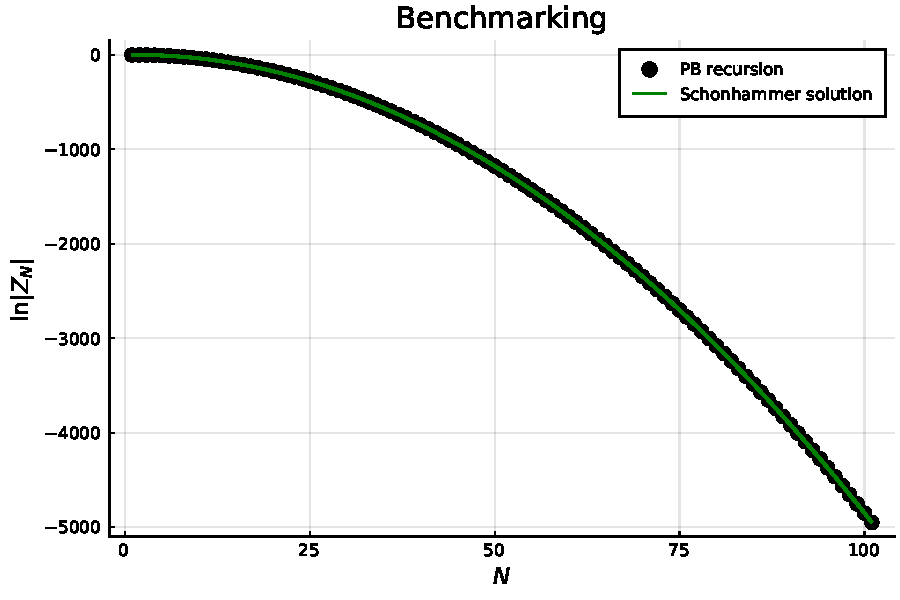
\includegraphics[scale=0.75]{figures/pdf/Benchmarking.pdf}
    \caption{Solution from Poisson Binomial recursive method versus the exact solution for the 1D simple harmonic oscillator. The black circles are the solutions from the Poisson Binomial recursion method. The green line is the exact solution using Sch\"onhammer's Eq.(\ref{schoneqn})}
    \label{fig: schon solution}
\end{figure}
\begin{figure}[H]
    \centering
    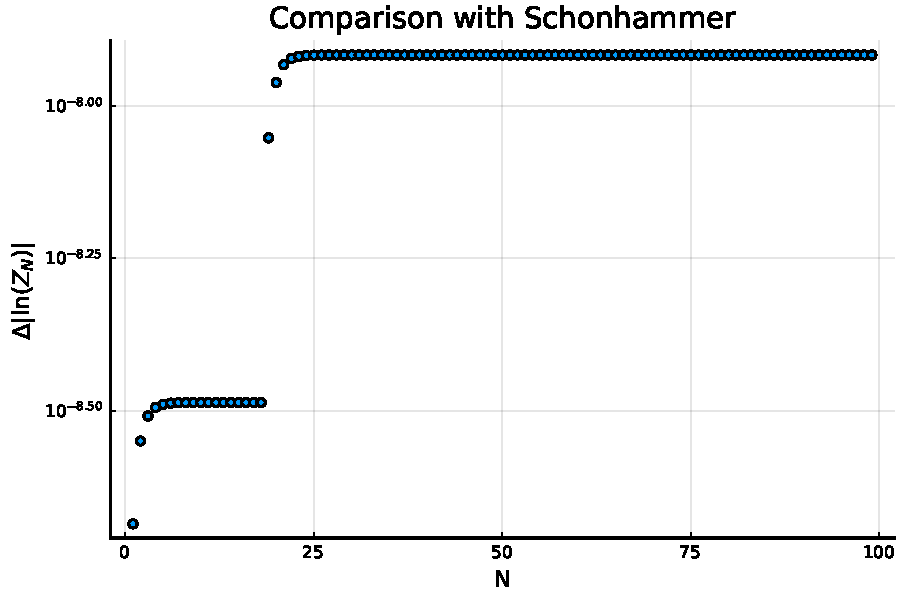
\includegraphics[scale=0.75]{figures/pdf/Benchdiff.pdf}
    \caption{The difference between the solutions presented in Fig. (\ref{fig: schon solution}). The precision of the Poisson binomial method was set to $10^{-8}$ which controls the range of the y-axis. The jump in error is due to the exclusion of terms below the Fermi level. Terms are chosen to be excluded if their occupation probability differs from one by a chosen cutoff value. In this case they are assumed to be in an occupied state. }
    \label{fig: schon diff}
\end{figure}

The other part to note is the jump in the error. This is due to the process of building the initial occupation probability distribution. As a reminder, the program is dealing with a fixed number of particles at ultra-low temperatures. At these temperatures, only the region around the Fermi level will have any sort of probability away from one or zero. Therefore, to increase the speed of the calculation, the states that are above a cutoff value are certain to be occupied. For these states with occupation probability of one, a counter keeps track of the number of particles and their probabilities are not included in the distribution. Similarly, any probability that is below the cutoff is not included because it is taken to have a zero probability of being occupied. This process saves memory and makes the calculations much faster. The downside to this process is that a small error is introduced. This is the source of the jump shown in Fig.\@ (\ref{fig: schon diff}). At this point, energy levels are left out of the distribution. Again, the error is controllable based on the precision chosen by the user.

\section{Controlling Chemical Potential}
The key role of the chemical potential is to ensure that the grand canonical ensemble has the correct number of particles in the system. The correct choice in chemical potential will affect the error of the measurement. Therefore, it's necessary to choose $\mu$ such that 
\begin{equation}
    \avg{N}=\sum_i \avg{p_i}
\end{equation}

where $N$ is the number of particles in the true canonical system. In the previous section, the partition function was calculated for different values of $N$. For each of these calculations, the choice in "fictitious" chemical potential is different. One interesting question is how much does this choice in chemical potential affect the error when calculating the partition function. To inspect this, we can set the chemical potential to a value and proceed with the same benchmarking code. The results of this are shown in Fig.\@ (\ref{fig:Errors}). We can see that the correct chemical potential will provide a minimum at its corresponding particle number value. After that, it increases as some absolute value of the distance from the correct $N$ value. Therefore, it is necessary that the chemical potential be updated each step in order to keep the errors at the minimum. 

\begin{figure}[H]
    \centering
    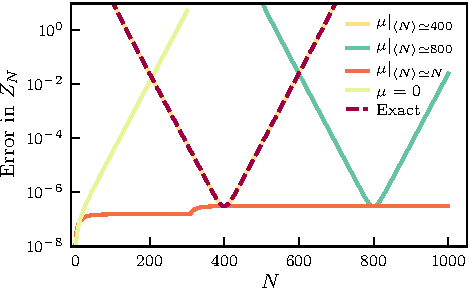
\includegraphics[scale=1.4]{figures/pdf/Plot1.pdf}
    \caption{The error associated with keeping the chemical potential $\mu$ fixed for a range of $N$ particles values. The accuracy of $\mu|_N$ is at the minimum error in a small range around $N$. The further $N$ is away from $\mu|_N$, the larger the error becomes. Therefore, it's necessary to recalculated $\mu$ for each value of $N$ in order to keep the error of the canonical partition function $Z_N$ to a minimum. This figure was provided by Jiangyong Yu. }
    \label{fig:Errors}
\end{figure}

\section{Numerical results of nondegenerate spectra}
In this section, we will consider the case where our spectrum is nondegenerate. From Section 1.4, we expect that the error of the temperature measurement $\beta^*$ in the grand canonical ensemble should reach $100\%$ once $\beta$ gets sufficiently large. We also saw the same result in Section 2.5.1 when $g_0=g_1=g_{-1}=...=1$ in Eq.\@ (\ref{filldegencheck}). We consider the simple harmonic oscillator (linear spectrum) and the potential well spectrum (quadratic spectrum). The numerical results are shown in Figs.\@ (\ref{fig:linnondeg}) and (\ref{fig:quadnondeg}) where the y-axis is $\frac{\delta\beta}{\beta}=\frac{\beta^*-\beta}{\beta}$. %An interesting difference between the two figures is length of the x-axis.
The linear spectrum reaches $100\%$ error slower than the quadratic error. This is due to the spacing between energy levels. For the linear spectrum, this spacing is constant, while the quadratic spectrum has a spacing that linearly increases. This means that more energy is required to fill the first excited state for the quadratic spectrum as the number of particles increases. The spacing term $\Delta_0$ will always increase, and thus the Boltzmann probability $e^{-\beta\Delta_0}$ that the state is occupied will continually decrease. For this reason, it is more difficult to calculate the error for linear spectra. 

\begin{figure}[H]
    \centering
    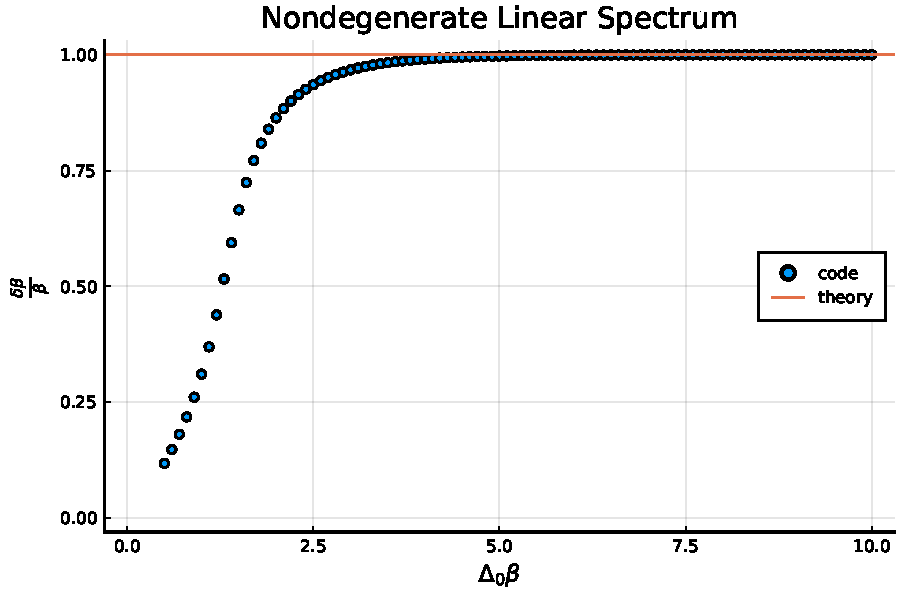
\includegraphics[scale=.75]{figures/pdf/linE_nondeg_N10.pdf}
    \caption{Error in $\beta^*$ measurement for a nondegenerate linear energy spectrum. Once $\Delta_0\beta$ is large enough, the error calculated from the code increases to $100\%$ as expected from the theory. }
    \label{fig:linnondeg}
\end{figure}

\begin{figure}[H]
    \centering
    \includegraphics[scale=0.75]{figures/pdf/quadE_nondeg_N10_Δ0=6.333.pdf}
    \caption{Error in $\beta^*$ measurement for a nondegenerate quadratic energy spectrum. Once $\Delta_0\beta$ is large enough, the error calculated from the code increases to $100\%$ as expected from the theory. }
    \label{fig:quadnondeg}
\end{figure}


\section{Numerical results of degenerate spectra}
In this section, we consider degenerate spectra. Specifically, we want to verify the equations in Section 2.5. We first consider the case where the Fermi level is filled and then consider the case of partial filling. Finally, we investigate a special case where the Fermi level is almost degenerate. 
\subsection{Filled Fermi Level}
To start, the linear energy spectrum is used. Eq.\@ (\ref{filldegen}) is compared with the results from the recursion calculation Fig.\@ (\ref{fig:Filled}).  

\begin{figure}[H]
    \centering
    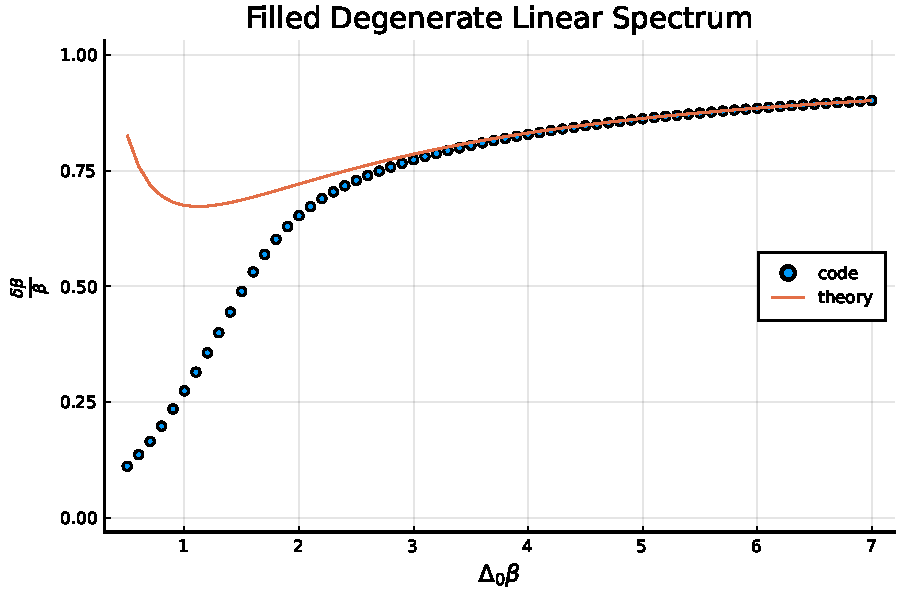
\includegraphics[scale=0.75]{figures/pdf/linE_filldegen_g0-2_N10.pdf}
    \caption{Error in $\beta^*$ measurement for a linear energy spectrum with a filled degenerate Fermi level. Once $\Delta_0\beta$ is large enough, the error calculated from the code follows the theoretical line in orange.}
    \label{fig:Filled}
\end{figure}

We can see that the error follows the theory once $\beta$ is sufficiently large. To further inspect this, consider rewriting Eq.\@ (\ref{filldegen}) in the following way. 
\begin{align}
    \frac{\delta\beta}{\beta}&=1-\frac{\ln(g_0g_1)}{\Delta_0\beta}\nonumber\\
    \frac{\delta\beta}{\beta}-1&=-\frac{\ln(g_0g_1)}{\Delta_0\beta}\nonumber\\
    \beta\Delta_0-\delta\beta\Delta_0&=\ln(g_0g_1) \label{3.2}
\end{align}
In this calculation, I have neglected the exponential term for convenience. Eq.\@ (\ref{3.2}) is then plotted against the program as shown in Fig. (\ref{fig:FilledDegenerateLinearSpectrumAdjustedError}). 
\begin{figure}[H]
    \centering
    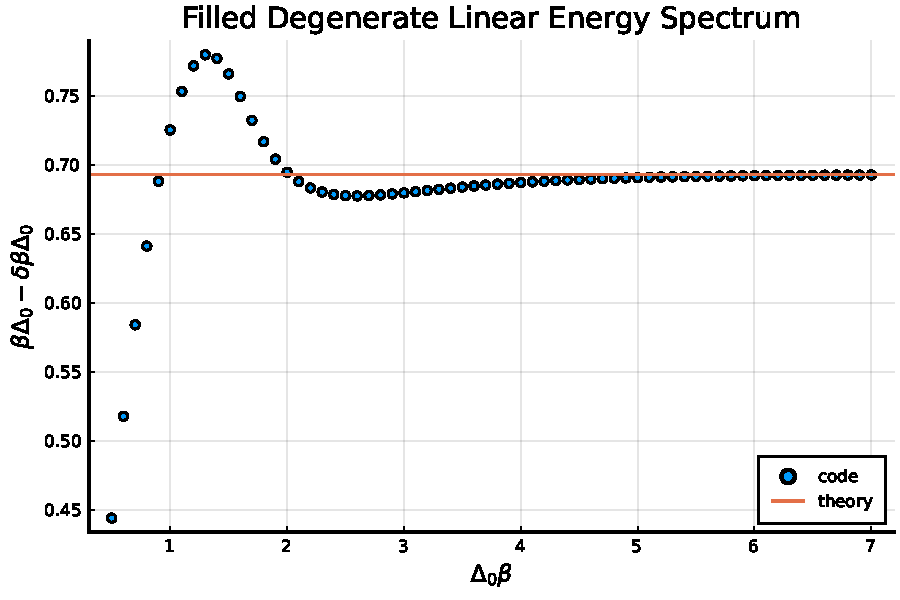
\includegraphics[scale=0.75]{figures/pdf/linE_filldegen_g0-2_N10_1.pdf}
    \caption{Error in $\beta^*$ measurement for a linear energy spectrum with a filled
degenerate Fermi level. The figure is adjusted to plot Eq.\@ (\ref{3.2}). Once $\Delta_0\beta$ is large enough, the $\ln(g_0g_1)$ limit is reached. For the case shown above, $g_0=2$ and $g_1=1$ so the asymptotic limit is $\ln(2)$ as shown in orange.}
    \label{fig:FilledDegenerateLinearSpectrumAdjustedError}
\end{figure}
Again, we can see that at high enough $\beta$ the program aligns with the theory. 

Now I will consider the filled degenerate quadratic energy spectrum. The analysis will be the same, so Eq.\@ (\ref{3.2}) will still be used. The results of the program are shown in Figs.\@ (\ref{fig:FilledDegenerate}) and (\ref{fig:FilledDegenerate2}). 

\begin{figure}[H]
    \centering
    \includegraphics[scale=0.75]{figures/pdf/quadE_filldegen_g0-2_N10_Δ0-7.pdf}
    \caption{Error in $\beta^*$ measurement for a quadratic energy spectrum with a filled
degenerate Fermi level. Once the temperature is small enough, the error calculated from the code
follows the theoretical line in orange.}
    \label{fig:FilledDegenerate}
\end{figure}

\begin{figure}[H]
    \centering
    \includegraphics[scale=0.75]{figures/pdf/quadE_filldegen_g0-2_N10_Δ0-7_1.pdf}
    \caption{Error in $\beta^*$ measurement for a quadratic energy spectrum with a filled
degenerate Fermi level. The figure is adjusted to plot Eq.\@ (\ref{3.2}). Once $\Delta_0\beta$ is large enough, the $\ln(g_0g_1)$ limit is reached. For the case shown above, $g_0=2$ and $g_1=1$ so the asymptotic limit is $\ln(2)$ as shown in orange.}
    \label{fig:FilledDegenerate2}
\end{figure}
Again, we can see that the program follows the trend of the theory. One note should be made for the slight variation at $\beta$ values of 1.5 or higher. The deviation is due to the cutoff that is used to determine the correct $\beta^*$. Overall, however, the theory and program agree very well for filled degenerate energy spectra.

\subsection{Partially Filled Degenerate Energy Spectra}
Turning to the case of partial filling, we want to verify Eq.\@ (\ref{partfilldegen}). Again, the simple harmonic oscillator will be considered first. The results are shown in Fig.\@ (\ref{fig:PartiallyFilledDegenerateLinearSpectrum}). 

\begin{figure}[H]
    \centering
    \includegraphics[scale=0.75]{figures/pdf/linE_partfilldegen_N9_g0-2_l-1_Δ0-1.pdf}
    \caption{Error in $\beta^*$ measurement for a linear energy spectrum with a partially filled Fermi level. Once $\Delta_0\beta$ is large enough, the error calculated from the code follows the theoretical line in orange.}
    \label{fig:PartiallyFilledDegenerateLinearSpectrum}
\end{figure}

We can see that there is pretty good agreement for large $\beta$ values. We can follow the same procedure as the filled spectrum and rewrite Eq. (\ref{partfilldegen}) to get
\begin{align}
    \frac{\delta\beta}{\beta}&=\frac{1}{\beta\Delta_0}\ln(\frac{g_0-\ell+1}{g_0-\ell})\nonumber\\
    \delta\beta \Delta_0&=\ln(\frac{g_0-\ell+1}{g_0-\ell}). \label{3.3}
\end{align}
Eq.\@ (\ref{3.3}) can be plotted against the program data as seen in Fig. (\ref{fig:PartiallyFilledDegenerateLinearSpectrumAdjustedError}). 

\begin{figure}[H]
    \centering
    \includegraphics[scale=0.75]{figures/pdf/linE_partfilldegen_N9_g0-2_l-1_Δ0-1_1.pdf}
    \caption{Error in $\beta^*$ measurement for a linear energy spectrum with a partially filled Fermi level. The figure is adjusted to plot Eq.\@ (\ref{3.3}). Once $\Delta_0\beta$ is large enough, the error calculated from the code follows the theoretical line in orange.}
    \label{fig:PartiallyFilledDegenerateLinearSpectrumAdjustedError}
\end{figure}
We can see that the program is following the theory when $\beta$ is large enough. Turning to the quadratic spectrum, the same calculations are plotted on Figs.\@ (\ref{fig:PartiallyFilledDegenerateQuadraticSpectrumError} and (\ref{fig:PartiallyFilledDegenerateQuadraticSpectrumAdjustedError}). 

\begin{figure}[H]
    \centering
    \includegraphics[scale=0.75]{figures/pdf/quadE_partfilldegen_g0-2_l-1_N9_Δ0-7.pdf}
    \caption{Error in $\beta^*$ measurement for a quadratic energy spectrum with a partially filled Fermi level. Once $\Delta_0\beta$ is large enough, the error calculated from the code follows the theoretical line in orange.}
    \label{fig:PartiallyFilledDegenerateQuadraticSpectrumError}
\end{figure}

\begin{figure}[H]
    \centering
    \includegraphics[scale=0.75]{figures/pdf/quadE_partfilldegen_g0-2_l-1_N9_Δ0-7_1.pdf}
    \caption{Error in $\beta^*$ measurement for a quadratic energy spectrum with a partially filled Fermi level. The figure is adjusted to plot Eq.\@ (\ref{3.3}). Once $\Delta_0\beta$ is large enough, the error calculated from the code follows the theoretical line in orange.}
    \label{fig:PartiallyFilledDegenerateQuadraticSpectrumAdjustedError}
\end{figure}

The data follows the theory very well with the cutoff error still appearing after about $\beta=1$. Overall, the theory and data for the partially filled spectra agree very well. 
\subsection{Almost Degenerate Energy Spectrum}

For this section, we will consider the case where the spectrum is almost degenerate. The spectrum that is being considered is one where the energy of the first excited state is much smaller than the second excited state, but not equal to the Fermi energy. This sort of spectrum is nondegenerate, but look like a partially filled degenerate Fermi level at small $\beta$. From a theory standpoint, we expect that the error will follow the case of the partially filled Fermi level until $\beta$ is large enough to break the pseudo-degeneracy. This will happen when $\beta$ is large enough to recover a two level system. At this point, the excitations from levels other than the nearest energy level will not contribute. The results of this are shown in Figs.\@ (\ref{fig:linE_almostdegen}) and (\ref{fig:quadE_almostdegen}). 
\begin{figure}[H]
    \centering
    \includegraphics[scale=0.75]{figures/pdf/linE_almostdegen_nondegen_g0-2_l-1_N10_Δ0-1.pdf}
    \caption{Error in $\beta^*$ measurement of a linear energy spectrum with an Fermi level that is almost degenerate. The error follows the partially filled degenerate Fermi level case shown in green until the $\Delta_0 \beta$ is large enough to break the degeneracy and return to the non-degenerate theory shown in purple.}
    \label{fig:linE_almostdegen}
\end{figure}

\begin{figure}[H]
    \centering
    \includegraphics[scale=0.75]{figures/pdf/quadE_almostdegen_nondegen_g0-2_l-1_N10_Δ0-6.333.pdf}
    \caption{Error in $\beta^*$ measurement of a quadratic energy spectrum with an Fermi level that is almost degenerate. The error follows the partially filled degenerate Fermi level case shown in green until the $\Delta_0 \beta$ is large enough to break the degeneracy and return to the non-degenerate theory shown in purple.}
    \label{fig:quadE_almostdegen}
\end{figure}
In these figures, the theory and the code for the partially filled Fermi level case are provided. This shows that the temperature follows the partially filled theory before the two level system is recovered.

    \chapter{Conclusions} \label{ch:conclusion}
In summary, I have presented a stable recursive method for calculating the canonical partition function for a low temperature non-interacting Fermi gas. This method utilizes the Poisson binomial recursion relation (Eq.\@ (\ref{pbrr})) to take the occupation probabilies in the grand canonical ensemble and map them to a canonical ensemble with $N$ particles (Eq.\@(\ref{Ztildetopb}). This method fixes the numerical instabilities that are present in previous methods of calculating the canonical partition function (Eq.\@ (\ref{Borrmann})) and agrees very well with exact solutions (Eq.\@ (\ref{schoneqn})). The agreement with Sch\"onhammer's exact result is shown in Fig.\@ (\ref{fig: schon solution}) with a controllable accuracy shown in Fig.\@ (\ref{fig: schon diff}). With a proper benchmark, this method is used to extract the error in temperature which is shown in Figs. (\ref{fig:linnondeg}-\ref{fig:quadE_almostdegen}). For the nondegenerate and degenerate cases, the theory and program agree very well proving the accuracy of each. 

Future work with this project would be to collaborate with experimentalists test the program on a variety of experimental data. This would be a great testing ground to see the full capability of the program. Through collaboration, improvements to the speed and numerical stability to the program could be found. It would give the experimentalists accurate results for their data and allow for correction to previously published data sets.

An indirect future application is to quantum Monte Carlo (QMC). A sign problem exists in (QMC) for fermions similar to the way that a sign problem showed up in Borrmann's equation (\ref{Borrmann}). There may be a similarity between the sources of these sign problems that would allow for a similar method to be developed for QMC. Along with this, the method of getting the canonical ensemble from the grand canonical ensemble may be applied to QMC calculations that are performed in the grand canonical ensemble, but apply to the canonical ensemble. 
    %%%%%%%%%%%%%%%%%%%%%%%%%%%%%%%%%%%%%%%%%%%%%%%%%%%%%%%%%%%%%%%%%%%%%%%%%%%%%%%%%%%%%%%%%%%%%%%%%%%%%
    % BIBLIOGRAPHY
    %%%%%%%%%%%%%%%%%%%%%%%%%%%%%%%%%%%%%%%%%%%%%%%%%%%%%%%%%%%%%%%%%%%%%%%%%%%%%%%%%%%%%%%%%%%%%%%%%%%%%
    \makeBibliographyPage % make the bibliography title page - can be edited in ut-thesis-template.tex
    \bibliographystyle{unsrt} % bibliography style - recommend using apalike-doi as it hyperlinks DOIs
    \bibliography{references/references-dissertation.bib} % references.bib included in the references directory
    %%%%%%%%%%%%%%%%%%%%%%%%%%%%%%%%%%%%%%%%%%%%%%%%%%%%%%%%%%%%%%%%%%%%%%%%%%%%%%%%%%%%%%%%%%%%%%%%%%%%%
    % APPENDIX - OPTIONAL - COMMENT IF NOT NEEDED
    %%%%%%%%%%%%%%%%%%%%%%%%%%%%%%%%%%%%%%%%%%%%%%%%%%%%%%%%%%%%%%%%%%%%%%%%%%%%%%%%%%%%%%%%%%%%%%%%%%%%%
    \makeAppendixPage   % make the appendix title page - can be edited in ut-thesis-template.tex
    \appendix
    \chapter{Solutions to the 1D Schr\"odinger Equation}
In one dimension, the time independent Schr\"odinger Equation is
\begin{equation}
    \mathcal{H}\psi=\frac{P^2}{2m}\psi(x)+V(x)\psi(x)=E\psi(x)
\end{equation}
where $\psi(x)$ is the wavefunction, $P$ is the momentum operator, $E$ is the energy eigenvalue, and $V(x)$ is the potential. This equation can be solved exactly for certain potentials. The momentum operator can be written in position space as 
\begin{equation}
P=\frac{\hbar}{i}\frac{d}{dx}    
\end{equation}
The Schr\"odinger equation then becomes
\begin{equation}
    \frac{-\hbar^2}{2m}\frac{d^2 \psi}{dx^2} + V(x) \psi=E\psi
\end{equation}
In the following two sections, the Harmonic Oscillator and the Infinite Well will be considered following the work of Griffiths \cite{Griffiths}.
\section{Harmonic Oscillator}
The harmonic oscillator has a potential that is defined as 
\begin{equation}
    V(x)=\frac{1}{2}m\omega^2 x^2
\end{equation}
Plugging this into the Schr\"odinger equation yields
\begin{equation}
    \frac{-\hbar^2}{2m}\frac{d^2}{dx^2}\psi+\frac{1}{2}m\omega^2 x^2\psi=E\psi
\end{equation}
This can be rewritten as 
\begin{equation}
    E\psi=\frac{1}{2m}\qty[\qty(\frac{\hbar}{i}\frac{d}{dx})^2+\qty(m\omega x)^2]\psi=\mathcal{H}\psi
\end{equation}
To calculate this, I will introduce the following operator
\begin{equation}
    a_{\pm}\equiv \frac{1}{\sqrt{2\hbar m \omega}} (\mp ip+m\omega x)
\end{equation}
The Schr\"odinger equation can be written in terms of this raising and lowering operator. To do so, consider that
\begin{align}
    a_-a_+&=\frac{1}{2\hbar m\omega} (ip+m\omega x)(-ip+m\omega x)\nonumber\\
    &=\frac{1}{2\hbar m\omega} [p^2+(m\omega x)^2-im\omega (xp-px)]\nonumber\\
    &=\frac{1}{2\hbar m\omega} [p^2+(m\omega x)^2]-\frac{i}{2\hbar}[x,p]\nonumber\\
    &=\frac{1}{2\hbar m\omega} [p^2+(m\omega x)^2]-\frac{i}{2\hbar}(i\hbar)\nonumber\\
    &=\frac{1}{2\hbar m\omega} [p^2+(m\omega x)^2]+\frac{1}{2}
\end{align}
where the commutator $[x,p]=xp-px=i\hbar$ was used in the fourth line. $a_-a_+$ can be substituted into Equation (A.6) to arrive at 
\begin{equation}
    \mathcal{H}=\hbar\omega\qty(a_-a_+-\frac{1}{2})
\end{equation}
Some properties of the ladder operators will help later calculations,
\begin{gather}
    [a_-,a_+]=1\\
    a_+\psi_n=\sqrt{n+1} \psi_{n+1}\\
    a_-\psi_n=\sqrt{n}\psi_{n-1}\\
    a_-\psi_0=0
\end{gather}
Using the commutator between the two operators, the Hamiltonian can also be written as 
\begin{equation}
    \mathcal{H}=\hbar\omega\qty(a_+a_-+\frac{1}{2})
\end{equation}
The energy spectrum can be calculated by finding the expectation value of this Hamiltonian. For convenience, let $\psi_n=\ket{n}$. This yields 
\begin{align}
    E=\avg{\mathcal{H}}&=\braket{n|\mathcal{H}|n}=\braket{n|\hbar\omega (a_+a_-+\frac{1}{2})|n}\nonumber\\
    &=\hbar\omega \braket{n|a_+a_-|n}+\frac{\hbar\omega}{2}\braket{n|n}\nonumber\\
    &=\hbar\omega \sqrt{n}\braket{n|a_+|n-1}+\frac{\hbar\omega}{2}\nonumber\\
    &=\hbar\omega n \braket{n|n}+\frac{\hbar\omega}{2}\nonumber\\
    &=\hbar\omega n +\frac{\hbar\omega}{2}\nonumber\\
    &=\hbar\omega(n+\frac{1}{2})
\end{align}
This is the equation for the energy spectrum of the simple harmonic oscillator. It is a linear equation in $n$, so it is called a linear energy spectrum. The energy spectrum can be seen in Figure (A.1).
\begin{figure}
    \centering
    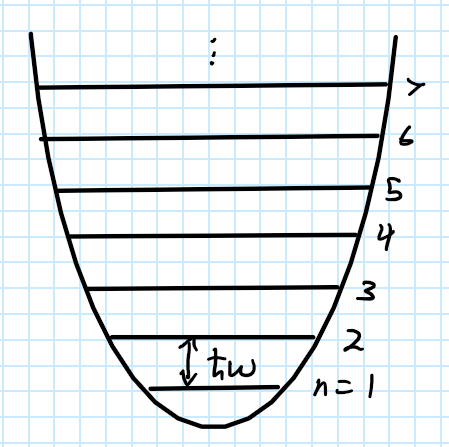
\includegraphics[scale=0.5]{figures/pdf/SHMspectrum.PNG}
    \caption{Simple Harmonic Oscillator Spectrum}
    \label{fig:Simple Harmonic Oscillator Spectrum}
\end{figure}Throughout this paper, any reference to a linear energy spectrum is directly a reference to the energy spectrum of a simple harmonic oscillator.

\section{Infinite Well}
The infinite square well is defined with a potential 
\begin{equation}
    V(x)=\begin{cases} 0 & 0\leq x \leq a\\
                       \infty & \text{otherwise}
        \end{cases}
\end{equation}
Plotting this potential shows the "well" shape that gives this potential its name. This is shown in Figure (A.2).
\begin{figure}
    \centering
    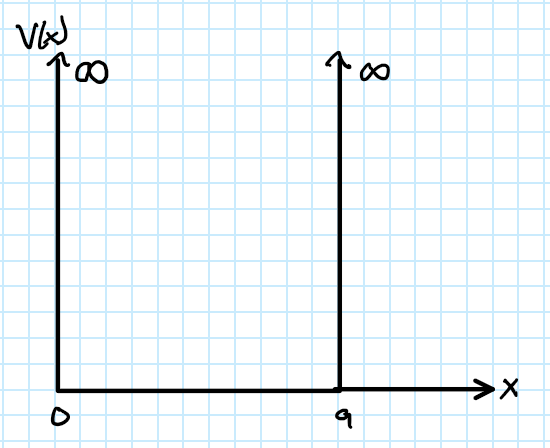
\includegraphics[scale=0.5]{figures/pdf/infsqpot.PNG}
    \caption{Infinite Well Potential}
    \label{fig: Infinite Well Potential}
\end{figure}
When plugging this potential into the Schr\"odinger equation, the only surviving part is when $V=0$. This means that there's one equation to solve with boundary conditions at $x=0,a$. Inserting the potential yields
\begin{align}
    -\frac{\hbar^2}{2m}\frac{d^2\psi}{dx^2}&=E\psi\nonumber\\
    \frac{d^2\psi}{dx^2}&=-\frac{2mE}{\hbar^2}\psi\nonumber\\
    \frac{d^2\psi}{dx^2}&=-k^2\psi
\end{align}
where $k=\frac{\sqrt{2mE}}{\hbar}$. The form of this equation is that of the classical simple harmonic oscillator, so $\psi$ can be directly written as 
\begin{equation}
    \psi=A\sin(kx)+B\cos(kx)
\end{equation}
The boundary condition at $x=0$ gives the $B$ constant 
\begin{align}
    \psi(0)=0&=A\sin(k(0))+B\cos(k(0))\\
    &=0+B\\
    B&=0
\end{align}
The other boundary condition gives
\begin{align}
    \psi(a)=0=A\sin(ka)
\end{align}
The trivial solution to this problem is $A=0$. This does not give any information about the energy spectrum, so instead consider the case where $A\neq 0$. This means that the $\sin(ka)$ term must be zero. This can only happen when $ka=n\pi$ where $n$ is an integer. Since $k$ is related to the energy, the spectrum can be found as
\begin{align}
    k=\frac{\sqrt{2mE}}{\hbar}&=\frac{n\pi}{a}\\
    E&=\frac{1}{2m} \qty(\frac{\hbar n\pi}{a})^2 
\end{align}
Since this equation is quadratic in $n$, it is called the quadratic energy spectrum. The spectrum is shown in Figure (A.3). Any reference to a quadratic spectrum in this paper is considering the energy spectrum in Equation (A.24)
\begin{figure}
    \centering
    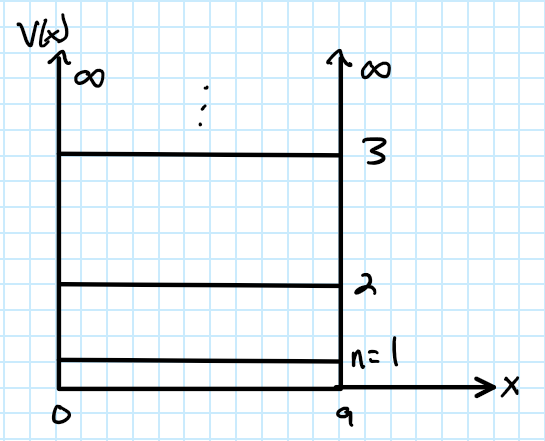
\includegraphics[scale=0.5]{figures/pdf/infsqspec.PNG}
    \caption{Energy spectrum of the infinite square well}
    \label{fig:Energy spectrum of the infinite square well}
\end{figure}
Turning back to the wave function, the value for $k$ can be plugged back into the equation for $psi$ giving
\begin{equation}
    \psi(x)=A\sin(\frac{n\pi}{a}x).
\end{equation}
The term $A$ is a normalization constant that is found by solving $\int|\psi(x)|^2 dx$. Doing this gives $A=\sqrt{\frac{2}{a}}$ and Equation (A.25) becomes 
\begin{equation}
    \psi(x)=\sqrt{\frac{2}{a}}\sin(\frac{n\pi}{a}x).
\end{equation}
    \chapter{$\chi^2$ derivatives}
The function, $\chi^2$, is defined as follows.
\begin{equation}
\chi^2=\sum_i(p_i-\avg{n_c}_i)^2
\end{equation}
The first derivative can be set to zero to find the minima and the second derivative will be used to determine if the zero values are at the the true minimum or at the tail end of this function. Solving the first derivative is done as follows.
\begin{gather}
    d\chi^2=\eval{\frac{\partial \chi^2}{\partial \beta^*}}_y d \beta^* 
    +\eval{\frac{\partial \chi^2}{\partial y}}_{\beta^*} d y\\    
    \frac{d\chi^2}{d\beta^*}=\eval{\frac{\partial \chi^2}{\partial 
    \beta^*}}_y +\frac{\partial \chi^2}{\partial y}\Biggr|_{\beta^*} 
    \frac{d y}{d \beta^*}
\end{gather}
The condition that the sum of $p_i$ must equal the total number of particles can be utilized to find the last term in the equation above. 
\begin{gather}
    dN=0=\eval{\frac{\partial N}{\partial \beta^*}}_y d \beta^* +\eval{\frac{\partial N}{\partial y}}_{\beta^*} d y\\
    \eval{\frac{\partial N}{\partial \beta^*}}_y d \beta^*=-\eval{\frac{\partial N}{\partial y}}_{\beta^*} d y\nonumber\\
    \frac{d y}{d \beta^*}=-\frac{\eval{\frac{\partial N}{\partial \beta^*}}_y}{\eval{\frac{\partial N}{\partial y}}_{\beta^*}}\\
    \eval{\frac{\partial N}{\partial \beta^*}}_y= \sum_i \frac{\partial p_i}{\partial \beta^*}=\sum_i \frac{-e^{\beta^* \epsilon_i-y}}{(1+e^{\beta^* \epsilon_i-y})^2}\epsilon_i=-\sum_i \epsilon_i p_i q_i\\
    \eval{\frac{\partial N}{\partial y}}_{\beta^*}=\frac{\partial p_i}{\partial y}=\sum_i -\frac{-e^{\beta^* \epsilon_i-y}}{(1+e^{\beta^* \epsilon_i-y})^2}=\sum_i p_i q_i\\
    \frac{d y}{d \beta^*}=-\frac{-\sum_i \epsilon_i p_i q_i}{\sum_i p_i q_i}=\frac{\sum_i \epsilon_i p_i q_i}{\sum_i p_i q_i}=C_1
\end{gather}
Turning back to the original equation, 
\begin{align}
    \eval{\frac{\partial \chi^2}{\partial \beta^*}}_y&=\sum_i 2(p_i-\avg{n_c}_i) \frac{-\epsilon_i e^{\beta^* \epsilon_i-y}}{1+e^{\beta^* \epsilon_i-y}}=\sum_i -2(p_i-\avg{n_c}_i)p_i q_i \epsilon_i\\
    \eval{\frac{\partial \chi^2}{\partial y}}_{\beta^*}&=\sum_i 2(p_i-\avg{n_c}_i) \frac{e^{\beta^* \epsilon_i-y}}{1+e^{\beta^* \epsilon_i-y}}=\sum_i 2(p_i-\avg{n_c}_i)p_i q_i\\
    0&=\frac{d\chi^2}{d\beta^*}=\sum_i -2(p_i-\avg{n_c}_i)p_i q_i \epsilon_i+\sum_i 2(p_i-\avg{n_c}_i)p_i q_i C_1\nonumber\\
    0&=\sum_i 2(p_i-\avg{n_c}_i)p_i q_i (\epsilon_i-C_1)\nonumber\\
    0&=\sum_i 2(p_i-\avg{n_c}_i)p_i q_i (\epsilon_i-\frac{\sum_k \epsilon_k p_k q_k}{\sum_k p_k q_k} )
\end{align}
The equation for the first derivative can be set equal to zero in order to find the minimum.

Before looking at the second derivative, it is beneficial to analyze the derivatives of the functions $p_i$ and $q_i$.
\begin{gather}
    \eval{\frac{\partial p_i}{\partial \beta^*}}_y=-\epsilon_i p_i q_i\\
    \eval{\frac{\partial p_i}{\partial y}}_{\beta^*}=p_i q_i\\
    \eval{\frac{\partial q_i}{\partial \beta^*}}_y=\frac{\epsilon_i e^{y- 
    \beta^* \epsilon_i}}{(e^{y-\beta^* \epsilon_i}+1)^2}=q_i p_i 
    \epsilon_i\\
    \eval{\frac{\partial q_i}{\partial y}}_{\beta^*}=\frac{-e^{y-\beta^* 
    \epsilon_i}}{(e^{y-\beta^* \epsilon_i}+1)^2}=-q_i p_i
\end{gather}
These will be useful for the calculations of the second derivative which is done as follows.  
\begin{gather}
    \frac{d}{d\beta^*} \qty{\frac{d \chi^2}{d\beta^*}} = \frac{\partial } 
    {\partial \beta^*} \eval{\qty{\frac{d \chi^2}{d\beta^*}}}_y+ 
    \frac{\partial }{\partial y} \eval{\qty{\frac{d \chi^2} 
    {d\beta^*}}}_{\beta^*} \frac{dy}{d\beta^*}\nonumber\\
    \frac{d}{d\beta^*} \qty{\frac{d \chi^2}{d\beta^*}} = \frac{\partial } 
    {\partial \beta^*} \eval{\qty{\frac{d \chi^2}{d\beta^*}}}_y+ 
    \frac{\partial }{\partial y} \eval{\qty{\frac{d \chi^2} 
    {d\beta^*}}}_{\beta^*} C_1
\end{gather}
Once again, each component needs to be calculated. The term $C_1$ is the same so the other two terms are the only ones to be calculated. Starting on the left equation,
\begin{align}
&\frac{\partial}{\partial \beta^*} \qty{\frac{d \chi^2}{d \beta^*}} =\frac{\partial}{\partial \beta^*} [-2\sum_i (p_i-\avg{n_c}_i)p_i q_i \epsilon_i+2\sum_i (p_i-\avg{n_c}_i)p_i q_i C_1]\\
    &\quad=-2\sum_i[p_i q_i \epsilon_i (-\epsilon_i p_i q_i) +(p_i-\avg{n_c}_i) q_i \epsilon_i(-\epsilon_i p_i q_i)+ (p_i-\avg{n_c}_i)p_i \epsilon_i(q_i p_i \epsilon_i)\nonumber\\
    &\quad+(-\epsilon_i p_i q_i) p_i q_i C_1+ (p_i-\avg{n_c}_i)(-\epsilon_i p_i q_i) q_i C_1+(p_i-\avg{n_c}_i)p_i(q_i p_i \epsilon_i) C_1\nonumber\\
    &\quad+ (p_i-\avg{n_c}_i) p_i q_i C_2]
\end{align}
Where $C_2$ is
\begin{align}
    C_2&=\frac{\partial C_1}{\partial \beta^*}=\frac{\partial}{\partial \beta^*} \frac{\sum_i p_i q_i \epsilon_i}{\sum_i p_i q_i}\nonumber\\
    &=\frac{\frac{\partial }{\partial \beta^*}(\sum_i \epsilon_i q_i p_i) \sum_i p_i q_i - \sum_i p_i q_i \epsilon_i \frac{\partial}{\partial \beta^*}(\sum_i p_i q_i)}{(\sum_i p_i q_i)^2}\nonumber\\
    &=\frac{[\sum_i \epsilon_i(-\epsilon_i p_i q_i)q_i + \sum_i \epsilon_i p_i (p_i q_i \epsilon_i)]\sum_k p_k q_k-\sum_k \epsilon_k p_k q_k[\sum_i \epsilon_i p_i q_i p_i+\sum_i q_i(-\epsilon_i p_i q_i)]}{(\sum_i p_i q_i)^2}\nonumber\\
    &=\frac{[-\epsilon_i^2p_i q_i^2+ \sum_i \epsilon_i^2 p_i^2 q_i]\sum_k p_k q_k-\sum_k \epsilon_k p_k q_k[\sum_i \epsilon_i p_i^2 q_i-\sum_i \epsilon_i p_i q_i^2]}{(\sum_i p_i q_i)^2}\nonumber\\
    &=\frac{\sum_i(\epsilon_i^2 p_i q_i(p_i-q_i))}{\sum_i p_i q_i}-\frac{\sum_k \epsilon_k p_k q_k}{(\sum_i p_i q_i)^2}(\sum_i \epsilon_i p_i q_i (p_i-q_i))\nonumber\\
    &=\frac{\sum_i(\epsilon_i^2 p_i q_i(p_i-q_i))}{\sum_i p_i q_i}-\frac{C_1(\sum_i \epsilon_i p_i q_i (p_i-q_i))}{\sum_i p_i q_i}\nonumber\\
    &=\frac{\sum_i \epsilon_i p_i q_i(p_i - q_i)(\epsilon_i-C_1)}{\sum_i p_i q_i}
\end{align}
For the other term, it can observe that the only difference between the $\beta^*$ derivative and $y$ is a factor of $-\epsilon_i$. Using this knowledge, the other term can be easily written as,
\begin{align}
    \frac{\partial}{\partial y}\qty{\frac{d\chi^2}{d\beta^*}}&=2 
    \sum_i (p_i-\avg{n_c}_i)\Biggr[(\epsilon_i-C_1)p_iq_i[p_i-q_i-p_iq_i]+p_iq_iC_3\Biggr]
\end{align}
where $C_3$ is (using the same factor of $-\epsilon_i$),
\begin{gather}
    C_3=\frac{\partial C_1}{\partial y}=\frac{\partial}{\partial 
    y}\qty{\frac{\sum_i \epsilon_i q_i p_i}{\sum_i p_i q_i}}=\frac{\sum_i p_i q_i(q_i-p_i)(\epsilon_i-C_1)}{\sum_i p_i q_i}
\end{gather}
With this, the full second derivative is
\begin{align}
&\frac{d}{d\beta^*} \qty{\frac{d \chi^2}{d\beta^*}} = \frac{\partial }{\partial \beta^*} \eval{\qty{\frac{d \chi^2}{d\beta^*}}}_y+ \frac{\partial }{\partial y} \eval{\qty{\frac{d \chi^2}{d\beta^*}}}_{\beta^*} C_1\nonumber\\
&\quad=2\sum_i\qty{(\epsilon_i-C_1)^2[(p_i-\avg{n_c}_i)p_iq_i(q_i-p_i)+p_i^2q_i^2]+(p_i-\avg{n_c}_i)p_iq_i(C_1C_3+C_2)}
\end{align}
    \chapter{Degeneracy Relationships}
\section{Filled Degenerate Spectrum}\label{section:c1}
For Section \ref{section:filleddegen} the relationship $\frac{\avg{n_0}_{g_0}}{1-\avg{n_0}_{g_0}}$ arises. Throughout the following calculations, only the leading order terms will be considered since $e^{-\beta\Delta_0}$ is sufficiently small at large $\beta$ .These values will be calculated here starting with the $\avg{n_0}_{g_0}$ term. Plugging in the value for $\avg{n_0}_{g_0}$ from Eq. (\ref{2.20}),
\begin{align}
    1-\avg{n_0}_{g_0}&=\frac{1+g_0g_1e^{-\beta\Delta_0}+\frac{g_0(g_0-1)g_1(g_1-1)}{4}e^{-2\beta\Delta_0}}{...}\nonumber\\
    & \ \ \ -\frac{1+(g_0-1)e^{-\beta\Delta_0}+\frac{(g_0-1)(g_0-2)g_1(g_1-1)}{4} e^{-2\beta\Delta_0}}{...}\nonumber\\
    &=\frac{g_1e^{-\beta^*\Delta_0}+\frac{(g_0-1)g_1(g_1-1)}{2}e^{-2\beta^*\Delta_0}}{...}\\
    \frac{\avg{n_0}_{g_0}}{1-\avg{n_0}_{g_0}}&=\frac{1+(g_0)g_1 e^{-\beta\Delta_0}}{g_1e^{-\beta^*\Delta_0}+\frac{(g_0-1)g_1(g_1-1)}{2}e^{-2\beta^*\Delta_0}}\nonumber\\
    &=\frac{1+(g_0)g_1 e^{-\beta\Delta_0}}{g_1e^{-\beta^*\Delta_0}(1+\frac{(g_0-1)(g_1-1)}{2}e^{-\beta^*\Delta_0})}.
\end{align}
Since $e^{-\beta\Delta_0}$ is sufficiently small, the denominator can be approximated using $(1+x)^{-1}\approx 1-x$. This gives
\begin{align}
    \frac{\avg{n_0}_{g_0}}{1-\avg{n_0}_{g_0}}&=\frac{e^{-\beta\Delta_0}}{g_1}\qty(1+(g_0-1)g_1e^{-\beta\Delta_0})\qty(1-\frac{(g_0-1)(g_1-1)}{2}e^{-\beta\Delta_0})\nonumber\\
    &=\frac{e^{-\beta\Delta_0}}{g_1} \qty(1+(g_0-1)g_1e^{-\beta\Delta_0}-\frac{(g_0-1)(g_1-1)}{2}e^{-\beta\Delta_0})\nonumber\\
    &=\frac{e^{-\beta\Delta_0}}{g_1} \qty(1+\frac{1}{2}(g_1+1)(g_0-1) e^{-\beta\Delta_0}).
\end{align} 
Squaring this quantity gives
\begin{align}
    \qty(\frac{\avg{n_0}_{g_0}}{1-\avg{n_0}_{g_0}})^2&=\frac{e^{2\beta\Delta_0}}{g_1^2}\qty(1+(g_1+1)(g_0-1)e^{-\beta\Delta_0}).
\end{align}

\section{Partially Filled Spectrum Chemical Potential} \label{section:c2}
The chemical potential is solved for using the particle number like in Eq. (\ref{2.24}). This develops into  
\begin{align}
    &g_{-1}+\ell=\frac{g_1}{1+e^{\beta(\Delta_1-\mu)}}+\frac{g_0}{1+e^{-\beta\mu}}+\frac{g_{-1}}{1+e^{\beta(\Delta_{-1}-\mu)}}\\
    &(g_{-1}+\ell)(1+e^{\beta(\Delta_1-\mu)})(1+e^{-\beta\mu})(1+e^{\beta(\Delta_{-1}-\mu)})=g_1(1+e^{-\beta\mu})(1+e^{\beta(\Delta_{-1}-\mu)})\nonumber\\
    &\quad+g_0(1+e^{\beta(\Delta_1-\mu)})(1+e^{\beta(\Delta_{-1}-\mu)})+g_{-1}(1+e^{\beta(\Delta_1-\mu)})(1+e^{-\beta\mu}).
    \end{align}
Starting with the left hand side,
\begin{align}
    &(g_{-1}+\ell)(1+e^{\beta(\Delta_1-\mu)})(1+e^{-\beta\mu})(1+e^{\beta(\Delta_{-1}-\mu)})\nonumber\\
    &\quad=(g_{-1}+\ell)(1+e^{-\beta\mu}(1+e^{\beta\Delta_1})+e^{-2\beta\mu}e^{\beta\Delta_1})(1+e^{\beta(\Delta_{-1}\beta})\nonumber\\
    &\quad=(g_{-1}+\ell)(1+e^{-\beta\mu}(1+e^{\beta\Delta_1})+e^{-2\beta\mu}e^{\beta\Delta_1}+e^{-2\beta\mu}e^{\beta\Delta_{-1}}(1+e^{\beta\Delta_1})\nonumber\\
    &\quad+e^{-3\beta\mu}e^{\beta(\Delta_1+\Delta_{-1})})\nonumber\\
    &\quad=(g_{-1}+\ell)(1+e^{-\beta\mu}(1+e^{\beta\Delta_1}+e^{\beta\Delta_{-1}})+e^{-2\beta\mu}(e^{\beta\Delta_1}+e^{\beta\Delta_{-1}}+e^{\beta(\Delta_{-1}+\Delta_1)})\nonumber\\
    &\quad+e^{-3\beta\mu}e^{\beta(\Delta_1+\Delta_{-1})}).
\end{align}
Next, the right hand side is
\begin{align}
    &g_1(1+e^{-\beta\mu})(1+e^{\beta(\Delta_{-1}-\mu)})+g_0(1+e^{\beta(\Delta_1-\mu)})(1+e^{\beta(\Delta_{-1}-\mu)})\nonumber\\
    &\quad+g_{-1}(1+e^{\beta(\Delta_1-\mu)})(1+e^{-\beta\mu})\label{C8}\\
    &\quad=g_1(1+e^{-\beta\mu}(1+e^{\beta\Delta_{-1}}+e^{\beta\Delta_{-1}}e^{-2\beta\mu}))\nonumber\\
    &\quad+g_0(1+e^{-\beta\mu}(e^{\beta\Delta_1}+e^{\beta\Delta_{-1}})+e^{-2\beta\mu}e^{\beta(\Delta_1+\Delta_{-1})})\nonumber\\
    &\quad+g_{-1}(1+e^{-\beta\mu}(1+e^{\beta\Delta_1})+e^{-2\beta\mu}e^{\beta\Delta_1}). \label{C9}
\end{align}
Combining both sides together yields,
\begin{align}
    &0=e^{-3\beta\mu}(e^{\beta(\Delta_1+\Delta_{-1})})\nonumber\\
    &\quad+e^{-2\beta\mu}(e^{\beta\Delta_1}+e^{\beta\Delta_{-1}}+e^{\beta(\Delta_{-1}+\Delta_1)}-\frac{g_1}{g_{-1}+\ell}e^{\beta\Delta_{-1}}\nonumber\\
    &\quad-\frac{g_0}{g_{-1}+\ell}e^{\beta(\Delta_1+\Delta_{-1})}-\frac{g_{-1}}{g_{-1}+\ell}e^{\beta\Delta_1})\nonumber\\
    &\quad+e^{-\beta\mu}(1+e^{\beta\Delta_1}+e^{\beta\Delta_{-1}}-\frac{g_1}{g_{-1}+\ell}(1+e^{\beta\Delta_{-1}})\nonumber\\
    &\quad-\frac{g_0}{g_{-1}+\ell}(e^{\beta\Delta_1}+e^{\beta\Delta_{-1}})-\frac{g_{-1}}{g_{-1}+\ell}(1+e^{\beta\Delta_1}))\nonumber\\
    &\quad+(1-\frac{g_1}{g_{-1}+\ell}-\frac{g_0}{g_{-1}+\ell}-\frac{g_{-1}}{g_{-1}+\ell}).
\end{align}

\section{Partially Filled Spectrum $\beta^*$ to $\beta$}\label{section:c3}
In Section \ref{section:partdegen}, it's necessary to write $e^{-\beta^*\Delta_0}$ in terms of $e^{-\beta\Delta_0}$. This is done by starting by setting Eq. (\ref{2.27}) equal to Eq. (\ref{2.42}). This becomes

\begin{align}
    &\frac{1-\avg{n_0}_\ell}{\avg{n_0}_\ell}=e^{-\beta^*\mu }=\frac{1}{2}((\frac{g_0}{\ell}-1)+(\frac{g_1}{\ell}-1)e^{-\beta^*\Delta_0})\\
    &\quad\quad +\frac{1}{2}\sqrt{((\frac{g_0}{\ell}-1)+(\frac{g_1}{\ell}-1)e^{-\beta^*\Delta_0})^2-4e^{-\beta^*\Delta_0}(1-\frac{g_0}{\ell}-\frac{g_1}{\ell})} \nonumber\\
    &\quad\qty[2\frac{1-\avg{n_0}_\ell}{\avg{n_0}_\ell}-\qty(\qty(\frac{g_0}{\ell}-1)+\qty(\frac{g_1}{\ell}-1)e^{-\beta^*\Delta_0})]^2=\nonumber\\
    &\quad\qty[\qty(\frac{g_1}{\ell}-1)+\qty(\frac{g_1}{\ell}-1)e^{-\beta^*\Delta_0}]^2-4e^{-\beta^*\Delta_0} \qty(1-\frac{g_0}{\ell}-\frac{g_1}{\ell})\\
    &4\qty(\frac{1-\avg{n_0}_\ell}{\avg{n_0}_\ell})^2-4 \frac{1-\avg{n_0}_\ell}{\avg{n_0}_\ell} \qty[\qty(\frac{g_0}{\ell}-1)+\qty(\frac{g_1}{\ell}-1)e^{-\beta^*\Delta_0}]\nonumber\\
    &\quad+\qty[\qty(\frac{g_0}{\ell}-1)+\qty(\frac{g_1}{\ell}-1)e^{-\beta^*\Delta_0}]^2= \qty[\qty(\frac{g_1}{\ell}-1)+\qty(\frac{g_1}{\ell}-1)e^{-\beta^*\Delta_0}]^2\nonumber\\
    &\quad -4e^{-\beta^*\Delta_0} \qty(1-\frac{g_0}{\ell}-\frac{g_1}{\ell})\nonumber\\
    &\quad e^{-\beta^*\Delta_0}\qty[\qty(\frac{g_1}{\ell}-1)(-4)\qty(\frac{1-\avg{n_0}_\ell}{\avg{n_0}_\ell})+4\qty(1-\frac{g_0}{\ell}-\frac{g_1}{\ell})]\nonumber\\
    &\quad =-4\qty(\frac{1-\avg{n_0}_\ell}{\avg{n_0}_\ell})^2+4\qty(\frac{1-\avg{n_0}_\ell}{\avg{n_0}_\ell})\qty(\frac{g_0}{\ell}-1).
\end{align}
This last equation can be written to get $\beta^*$ alone. This becomes 
\begin{align}
    e^{-\beta^*\Delta_0}&=\frac{\frac{1-\avg{n_0}_\ell}{\avg{n_0}_\ell}\qty(\frac{g_0}{\ell}-1)-\qty(\frac{1-\avg{n_0}_\ell}{\avg{n_0}_\ell})^2}{\qty(1-\frac{g_0}{\ell}-\frac{g_1}{\ell})-\qty(\frac{1-\avg{n_0}_\ell}{\avg{n_0}_\ell})\qty(\frac{g_1}{\ell}-1)}\\
    e^{\beta^*\Delta_0}&=\frac{\qty(1-\frac{g_0}{\ell}-\frac{g_1}{\ell})-\qty(\frac{1-\avg{n_0}_\ell}{\avg{n_0}_\ell})\qty(\frac{g_1}{\ell}-1)}{\frac{1-\avg{n_0}_\ell}{\avg{n_0}_\ell}\qty(\frac{g_0}{\ell}-1)-\qty(\frac{1-\avg{n_0}_\ell}{\avg{n_0}_\ell})^2}\nonumber\\
    &=\frac{\qty(\frac{\avg{n_0}_\ell}{1-\avg{n_0}_\ell})^2\qty(1-\frac{g_0}{\ell}-\frac{g_1}{\ell})-\qty(\frac{g_1}{\ell}-1)\qty(\frac{\avg{n_0}_\ell}{1-\avg{n_0}_\ell})}{\qty(\frac{g_0}{\ell}-1)\qty(\frac{\avg{n_0}_\ell}{1-\avg{n_0}_\ell})-1}\nonumber\\
    &=\frac{\qty(\frac{\avg{n_0}_\ell}{1-\avg{n_0}_\ell})^2(g_0+g_1-\ell)+(g_1-\ell)\qty(\frac{\avg{n_0}_\ell}{1-\avg{n_0}_\ell})}{\ell-(g_0-\ell)\qty(\frac{\avg{n_0}_\ell}{1-\avg{n_0}_\ell})}\nonumber\\
    &=\frac{\avg{n_0}_\ell^2(g_0+g_1-\ell)+(g_1-\ell)(\avg{n_0}_\ell-\avg{n_0}_\ell^2}{\ell(1-\avg{n_0}_\ell)^2-(\avg{n_0}_\ell-\avg{n_0}_\ell^2)(g_0-\ell)}\nonumber\\
    &=\frac{\avg{n_0}_\ell\qty(\avg{n_0}_\ell g_0+\avg{n_0}_\ell g_1-\avg{n_0}_\ell \ell+g_1-g_1\avg{n_0}_\ell-\ell+\ell\avg{n_0}_\ell)}{\ell(1-\avg{n_0}_\ell)-g_0(\avg{n_0}_\ell-\avg{n_0}_\ell^2)}\nonumber\\
    &=\frac{\avg{n_0}_\ell(g_1-\ell+g_0\avg{n_0}_\ell)}{(\ell-g_0\avg{n_0}_\ell)(1-\avg{n_0}_\ell)}\\
    e^{-\beta^*\Delta_0}&=\frac{\qty(\frac{\ell}{g_0}-\avg{n_0}_\ell)\qty(1-\avg{n_0}_\ell)}{\avg{n_0}_\ell\qty(\frac{g_1-\ell}{g_0}+\avg{n_0}_\ell)}. \label{C.16}
\end{align}
This equation can be solved by breaking it down into parts. The first part is  
\begin{align}
    \frac{\ell}{g_0}-&\avg{n_0}_\ell=\frac{\ell}{g_0}-\frac{\ell}{g_0}\qty(1-\frac{g_1}{g_0-\ell+1}e^{-\beta\Delta_0}+\frac{g_1(g_0-\ell+1)(g_1+\ell-1)+g_1^2 \ell}{(g_0-\ell+1)^2(g_0-\ell+2)} e^{-2\beta\Delta_0})\nonumber\\
    &=\frac{\ell g_1}{g_0(g_0-\ell+1)}e^{-\beta\Delta_0}\qty(1-\frac{(g_0-\ell+1)(g_1+\ell-1)+g_1\ell}{(g_0-\ell+1)(g_0-\ell+2)}e^{-\beta\Delta_0})\nonumber
\end{align}
\begin{align}
    &\frac{g_1-\ell}{g_0}+\avg{n_0}_\ell=\avg{n_0}_\ell+\frac{\ell}{g_0}\Biggr(1-\frac{g_1}{g_0-\ell+1}e^{-\beta\Delta_0}\nonumber\\
    &\quad\quad\quad+\frac{g_1(g_0-\ell+1)(g_1+\ell-1)+g_1^2 \ell}{(g_0-\ell+1)^2(g_0-\ell+2)} e^{-2\beta\Delta_0}\Biggr)\nonumber\\
    &\quad=\frac{g_1}{g_0}\qty[1-\frac{\ell}{g_0-\ell+1}e^{-\beta\Delta_0}+\frac{\ell(g_0-\ell+1)(g_1+\ell-1)+g_1\ell^2}{(g_0-\ell+1)^2(g_0-\ell+2)} e^{-2\beta\Delta_0}].
\end{align}
So the first three terms can be calculated as 
\begin{align}
    \frac{\frac{\ell}{g_0}-\avg{n_0}_\ell}{\avg{n_0}_\ell\qty(\avg{n_0}_\ell+\frac{g_1-\ell}{g_0})}&=\frac{\frac{\ell g_1}{g_0(g_0-\ell+1)}e^{-\beta\Delta_0}\qty[1-\frac{(g_0-\ell+1)(g_1+\ell-1)+g_1\ell}{(g_0-\ell+1)(g_0-\ell+2)}e^{-\beta\Delta_0}]}{\frac{g_1}{g_0}\qty[1-\frac{\ell}{g_0-\ell+1} e^{-\beta\Delta_0}]\frac{\ell}{g_0}\qty[1-\frac{g_1}{g_0-\ell+1} e^{-\beta\Delta_0}]}\nonumber\\
    &=\frac{\frac{g_0}{g_0-\ell+1}e^{-\beta\Delta_0}\qty[1-\frac{(g_0-\ell+1)(g_1+\ell-1)+g_1\ell}{(g_0-\ell+1)(g_0-\ell+2)}e^{-\beta\Delta_0}]}{1-\frac{g_1}{g_0-\ell+1}e^{-\beta\Delta_0}-\frac{\ell}{g_0-\ell+1}e^{-\beta\Delta_0}}\nonumber\\
    =\frac{g_0}{g_0-\ell+1}&e^{-\beta\Delta_0}\qty[1-\frac{(g_0-\ell+1)(g_1+\ell-1)+g_1\ell}{(g_0-\ell+1)(g_0-\ell+2)}e^{-\beta\Delta_0}]\nonumber\\
    &\quad\quad\quad\times\qty[1+e^{-\beta\Delta_0} \frac{g_1+\ell}{g_0-\ell+1}].
\end{align}
Here, only the terms that are first order in $e^{\beta\Delta_0}$ will be kept from the product of the two brackets. This gives
\begin{align}
    &=\frac{g_0}{g_0-\ell+1}e^{-\beta\Delta_0}\qty[1+e^{-\beta\Delta_0}\qty(\frac{g_1+\ell}{g_0-\ell+1}-\frac{(g_0-\ell+1)(g_1+\ell-1)+g_1\ell}{(g_0-\ell+1)(g_0-\ell+2)})]\nonumber\\
    &=\frac{g_0}{g_0-\ell+1}e^{-\beta\Delta_0}\qty[1+e^{-\beta\Delta_0}\qty(\frac{(g_0-\ell+1)+g_1+\ell-g_1\ell}{(g_0-\ell+1)(g_0-\ell+2)})].
\end{align}
The final term is
\begin{align}
    &1-\avg{n_0}_\ell=1-\frac{\ell}{g_0}\qty[1-\frac{g_1}{g_0-\ell+1}e^{-\beta\Delta_0}-\frac{g_1(g_0-\ell+1)(g_1+\ell-1)+g_1^2\ell}{(g_0-\ell+1)^2(g_0-\ell+2)}e^{-2\beta\Delta_0}]\nonumber\\
    &=\frac{g_0-\ell}{g_0}\qty[1-\frac{g_1\ell}{g_0-\ell+1}e^{-\beta\Delta_0}-\frac{\ell g_0g_1(g_0-\ell+1)(g_1+\ell-1)+g_1^2\ell^2}{(g_0-\ell)(g_0-\ell+1)^2(g_0-\ell+2)}e^{-2\beta\Delta_0}].
\end{align}
So the whole thing becomes 
\begin{align}
    &e^{-\beta^*\Delta_0}=\frac{g_0-\ell}{g_0}\qty(1+\frac{g_1\ell}{(g_0-\ell)(g_0-\ell+1)}e^{-\beta\Delta_0})\frac{g_0}{g_0-\ell+1}\nonumber\\
    &\quad\times e^{-\beta\Delta_0}\qty[1+\frac{(g_0-\ell+1)-g_1\ell+g_1+g_0}{(g_0-\ell+1)(g_0-\ell+2)}e^{-\beta\Delta_0}]\nonumber\\
    &\quad=\frac{g_0-\ell}{g_0-\ell+1}e^{-\beta\Delta_0}\Biggr(1+\frac{g_1\ell}{(g_0-\ell)(g_0-\ell+1)}e^{-\beta\Delta_0}\nonumber\\
    &\quad\quad +\frac{(g_0-\ell+1)-g_1\ell+g_1+g_0}{(g_0-\ell+1)(g_0-\ell+2)}e^{-\beta\Delta_0}\Biggr).
\end{align}
    %%%%%%%%%%%%%%%%%%%%%%%%%%%%%%%%%%%%%%%%%%%%%%%%%%%%%%%%%%%%%%%%%%%%%%%%%%%%%%%%%%%%%%%%%%%%%%%%%%%%%
    % A VITA IS REQUIRED
    %%%%%%%%%%%%%%%%%%%%%%%%%%%%%%%%%%%%%%%%%%%%%%%%%%%%%%%%%%%%%%%%%%%%%%%%%%%%%%%%%%%%%%%%%%%%%%%%%%%%%
    \addToTOC{Vita}
    \chapter*{Vita} \label{ch:vita}
\section*{Education}

\textbf{Masters of Science}, Physics, University of Tennessee, Knoxville, Knoxville, TN. Specialization:  Condensed Matter Physics. Master's Project: \emph{Low Temperature Thermometry}. May, 2022.

\noindent\textbf{Bachelor of Science}, Physics, Butler University, Indianapolis, In. May 2020.

\noindent\textbf{Bachelor of Science}, Electrical Engineering, IUPUI-Purdue School of Engineering and Technology, Indianapolis, In. May 2020. 
\end{document}
